\documentclass{article}

% if you need to pass options to natbib, use, e.g.:
% \PassOptionsToPackage{numbers, compress}{natbib}
% before loading nips_2017
%
% to avoid loading the natbib package, add option nonatbib:
% \usepackage[nonatbib]{nips_2017}

\usepackage{nips_2017}
\usepackage{dsfont}
% to compile a camera-ready version, add the [final] option, e.g.:
% \usepackage[final]{nips_2017}

\usepackage[utf8]{inputenc} % allow utf-8 input
\usepackage[T1]{fontenc}    % use 8-bit T1 fonts
\usepackage{hyperref}       % hyperlinks
\usepackage{url}            % simple URL typesetting
\usepackage{booktabs}       % professional-quality tables
\usepackage{amsfonts}       % blackboard math symbols
\usepackage{nicefrac}       % compact symbols for 1/2, etc.
\usepackage{microtype}      % microtypography

\usepackage{graphicx} % more modern
%\usepackage{epsfig} % less modern
%\usepackage{subfig} 
\usepackage{fancyvrb}

\usepackage{caption}
\usepackage{subcaption}

\fvset{fontsize=\footnotesize}


\usepackage{multirow}
\usepackage{array}

\usepackage{amssymb}
\usepackage{listings}
\usepackage{wrapfig}
\usepackage{tabularx}


\usepackage{verbatim}
 \usepackage{booktabs}
 % For algorithms
\usepackage{algorithm}
\usepackage{algorithmic}
\usepackage{tikz}
\usetikzlibrary{fit}
\usetikzlibrary{arrows.meta}
\usetikzlibrary{positioning}
\usetikzlibrary{decorations.text}
\usetikzlibrary{decorations.pathmorphing}

% As of 2011, we use the hyperref package to produce hyperlinks in the
% resulting PDF.  If this breaks your system, please commend out the
% following usepackage line and replace \usepackage{icml2016} with
% \usepackage[nohyperref]{icml2016} above.
\usepackage{amsmath}
\usepackage{hyperref}
\DeclareMathOperator*{\argmin}{arg\,min} % thin space, limits underneath in displays
% \DeclareMathOperator{\argmin}{argmin} % no space, limits underneath in displays
\DeclareMathOperator*{\argmax}{arg\,max} % thin space, limits underneath in displays
% \DeclareMathOperator{\argmax}{argmax} % no space, limits underneath in displays

\newcommand{\expect}{\mathds{E}} %{{\rm I\kern-.3em E}}
\newcommand{\probability}{\mathds{P}} %{{\rm I\kern-.3em P}}

\newcommand{\remark}[1]{\textcolor{red}{[#1]}}


% \title{Inferring Graphics Programs from Images}
\title{Learning to Infer Graphics Programs from Hand-Drawn Images}

% The \author macro works with any number of authors. There are two
% commands used to separate the names and addresses of multiple
% authors: \And and \AND.
%
% Using \And between authors leaves it to LaTeX to determine where to
% break the lines. Using \AND forces a line break at that point. So,
% if LaTeX puts 3 of 4 authors names on the first line, and the last
% on the second line, try using \AND instead of \And before the third
% author name.

\author{
  David S.~Hippocampus\thanks{Use footnote for providing further
    information about author (webpage, alternative
    address)---\emph{not} for acknowledging funding agencies.} \\
  Department of Computer Science\\
  Cranberry-Lemon University\\
  Pittsburgh, PA 15213 \\
  \texttt{hippo@cs.cranberry-lemon.edu} \\
  %% examples of more authors
  %% \And
  %% Coauthor \\
  %% Affiliation \\
  %% Address \\
  %% \texttt{email} \\
  %% \AND
  %% Coauthor \\
  %% Affiliation \\
  %% Address \\
  %% \texttt{email} \\
  %% \And
  %% Coauthor \\
  %% Affiliation \\
  %% Address \\
  %% \texttt{email} \\
  %% \And
  %% Coauthor \\
  %% Affiliation \\
  %% Address \\
  %% \texttt{email} \\
}

\begin{document}
% \nipsfinalcopy is no longer used

\maketitle

\begin{abstract}
  We introduce a model that learns to convert simple hand drawings
  into graphics programs written in a subset of \LaTeX.~The model
  combines techniques from deep learning and program synthesis.  We
  learn a convolutional neural network that proposes plausible drawing primitives
  that explain an image. This set of drawing primitives is like an execution trace for a graphics program. From this trace we use
  program synthesis techniques to recover a graphics
  program with constructs like variable bindings, iterative loops, or
  simple kinds of conditionals. With a graphics program in hand,
  we can correct errors made by the deep network, cluster drawings by use of similar high-level geometric structures, and extrapolate drawings.
  Taken together these results are a step towards
  agents that induce useful, human-readable programs from perceptual input.  
\end{abstract}

\section{Introduction}

 How can an agent convert noisy, high-dimensional perceptual input
 to a symbolic, abstract object, such as a computer program?  Here we
 consider this problem within a graphics program synthesis domain.  We
 develop an approach for converting natural images, such as hand
 drawings, into executable source code for drawing the original image.
 The graphics programs in our domain draw simple figures like those found in
 machine learning papers (see Figure~\ref{firstPageExamples}).
 %% \remark{The use of `graphics programs / visual programs' in the paper
 %%   title, title of this section, and the body of this section feels
 %%   too broad. `Graphics program' could conjur a lot of different ideas
 %%   (esp. 3D graphics); don't want to set the reader up to expect one
 %%   thing and then be disappointed that what you've done isn't
 %%   that. You bring up diagram-drawing later in the intro; I think it
 %%   should be made clear sooner (and certainly mentioned explicitly in
 %%   the abstract, when you get around to writing that).}

\newcommand{\exampleImageSize}{2cm}
\begin{figure}[h]
  \begin{minipage}[t]{0.7\linewidth}  
\begin{tabular}{llll}
  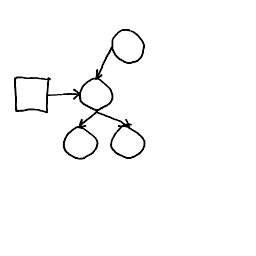
\includegraphics[width = \exampleImageSize]{figures/expert-60.png}&
  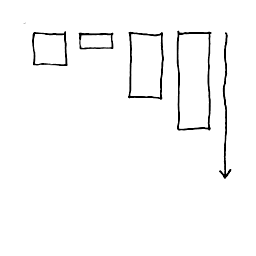
\includegraphics[width = \exampleImageSize]{figures/expert-5.png}&
    \includegraphics[width = \exampleImageSize]{figures/expert-17.png}&
    \includegraphics[width = \exampleImageSize]{figures/expert-58.png}\\
  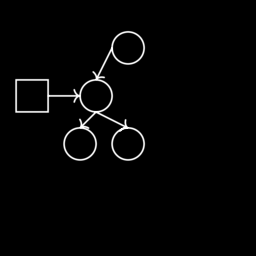
\includegraphics[width = \exampleImageSize]{figures/60.png}&
  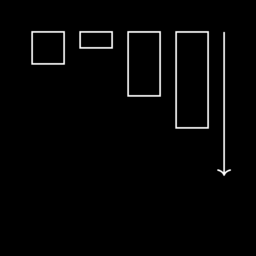
\includegraphics[width = \exampleImageSize]{figures/5.png}&
    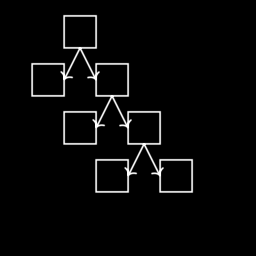
\includegraphics[width = \exampleImageSize]{figures/17.png}&
    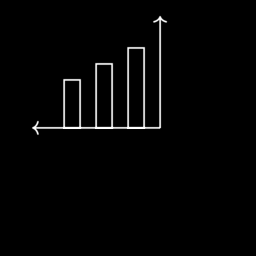
\includegraphics[width = \exampleImageSize]{figures/58.png}
\end{tabular}
\subcaption{}
  \end{minipage}%
  \begin{minipage}[t]{0.3\linewidth}
    \begin{tikzpicture}
      \node(picture) at (0,0) {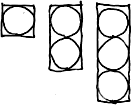
\includegraphics[width = 2cm]{figures/expert-31.png}};
      \draw[very thick,->] (picture.south)  -- (0,-2);
    \end{tikzpicture}\\
    \begin{minipage}[t]{0.3\linewidth}
\begin{verbatim}
for (i < 3)
 rectangle(3*i,-2*i + 4,
           3*i + 2,6)
 for (j < i + 1)
  circle(3*i + 1,-2*j + 5)
\end{verbatim}      
      \end{minipage}
    \subcaption{}
  \end{minipage}
  \caption{(a): Model learns to convert hand drawings (top) into \LaTeX~(bottom). (b) Synthesizes high-level \emph{graphics program} from hand drawing.}\label{firstPageExamples}
  \end{figure}

High dimensional perceptual input may seem ill matched to the abstract
semantics of a programming language. But programs with constructs such as
recursion or iteration produce a simpler \emph{execution trace} of
primitive actions; for our domain, the primitive actions are drawing
commands. Our hypothesis is that the execution trace of the program is
better aligned with the perceptual input, and that the trace can act
as a kind of bridge between perception and programs. We test this
hypothesis by developing a model that learns to map from an image to
the execution trace of the graphics program that drew it.  With the
execution trace in hand, we can bring to bear techniques from the
program synthesis community to recover the latent graphics program.
This family of techniques, called \emph{constraint-based program synthesis}~\cite{solar2008program},
work by modeling a set of possible programs inside of a constraint solver,
such as a SAT or SMT solver~\cite{de2008z3}.
These techniques excel at uncovering high-level symbolic structure,
but are not well equipped to deal with real-valued perceptual inputs.


We develop a hybrid architecture for inferring graphics programs.  Our
approach uses a deep neural network infer an execution trace from an
image; this network recovers primitive drawing operations such as
lines, circles, or arrows, along with their parameters. For added
robustness, we use the deep network as a proposal distribution for a
stochastic search over execution traces.  Section~\ref{neuralNetworkSection} describes this first stage of the architecture where we infer drawing commands from images, and explains how we handle noisy hand drawings.
Finally, we use program synthesis techniques to recover the program from its
trace.  The program synthesizer discovers constructs such as loops and
geometric operations such as reflections and affine transformations.
% \remark{This paragraph is all about making things a bit more
Section~\ref{programSynthesisSection} describes how the architecture
synthesizes programs from execution traces,
and how those programs are used for  correcting errors made by the deep network, measuring similarity between hand drawings,
and extrapolating figures.


%   so you really need more specifics about program synth here.}

%% Each of these three components -- the deep network, the stochastic
%% search, the program synthesizer -- confers its own advantages. From
%% the deep network, we get a fast system that can recover plausible
%% execution traces in about a minute~\remark{A minute seems slow to me, for deep net inference...}. From the stochastic search, we get
%% added robustness: essentially, the stochastic search can correct
%% mistakes made by the deep network's proposals.  From the program
%% synthesizer, we get abstraction: our system recovers coordinate
%% transformations, for loops, and subroutines, which are useful for
%% downstream tasks and can help correct some mistakes of the earlier stages.
%% % \remark{I wonder if this would work even better as a bulleted list...}
%% \remark{Tie these claims into the paper results: state what the `downstream' tasks are that you actually do, and refer to the sections where they occur}


\section{Related work}

Our work bears resemblance to the Attend-Infer-Repeat (AIR) system, which learns to decompose an image into its constituent objects~\cite{eslami1603attend}. AIR learns an iterative inference scheme which infers objects one by one and also decides when to stop inference; this is similar to our approach's first stage, which parses images into program execution traces. Our approach further produces interpretable, symbolic programs which generate those execution traces. The two approaches also differ in their architectures and training regimes: AIR learns a recurrent auto-encoding model via variational inference, whereas our parsing stage learns an autoregressive-style model from randomly-generated (execution trace, image) pairs. Finally, while AIR was evaluated on multi-MNIST images and synthetic 3D scenes, we focus on parsing and interpreting hand-drawn sketches.
% attend infer repeat:~\cite{eslami1603attend}. Crucial distinction is
% that they focus on learning the generative model jointly with the
% inference network. Advantages of our system is that we learn symbolic
% programs, and that we do it from hand sketches rather than synthetic
% renderings.

Our image-to-execution-trace parsing architecture builds on prior work on controlling procedural graphics programs~\cite{ritchie2016neurally}. Given a program which generates random 2D recursive structures such as vines, that system learns a structurally-identical ``guide program'' whose output can be directed, via neural networks, to resemble a given target image. 
We adapt this method to a different visual domain (figures composed of multiple objects), using a broad prior over possible scenes as the initial program and viewing the execution trace through the guide program as a symbolic parse of the target image.
We then show how to synthesize higher-level programs from these execution traces.

In the computer graphics literature, there have been other systems which convert sketches into procedural representations. One uses a convolutional network to match a sketch to the output of a parametric 3D modeling system~\cite{huang2017shape}. Another uses convolutional networks to support sketch-based instantiation of procedural primitives within an interactive architectural modeling system~\cite{Nishida:2016:ISU:2897824.2925951}. Both systems focus on inferring fixed-dimensional parameter vectors. In contrast, we seek to automatically infer a structured, programmatic representation of a sketch which captures higher-level visual patterns.

Prior work has also applied sketch-based program synthesis to authoring graphics programs. In particular, Sketch-n-Sketch presents a bi-directional editing system in which direct manipulations to a program's output automatically propagate to the program source code~\cite{Hempel:2016:SSP:2984511.2984575}. We see this work as complementary to our own: programs produced by our method could be provided to a Sketch-n-Sketch-like system as a starting point for further editing.

The CogSketch~\cite{forbus2011cogsketch} system also aims to have a
high-level understanding of hand-drawn figures. Their primary goal is
cognitive modeling (eg, they apply their system to solving IQ-test
style visual reasoning problems), whereas we are interested in
building an automated AI application (eg, in our system the user need
not annotate which strokes correspond to which shapes; our neural
network produces something equivalent to the annotations).  A key
similarity however is that both CogSketch and our system have as a
goal to make it easier to produce nice-looking figures.
Unsupervised Program Synthesis~\cite{ellis2015unsupervised} is a related framework which was also applied to geometric reasoning problems. The goals of~\cite{ellis2015unsupervised} were cognitive modeling,
and they applied their technique to synthetic scenes used in human behavioral studies.
%% open domain sketch understanding. structure mapping style model. also taps into cyc? the user segments the ink and labels them with concepts from knowledge base. like us they focus on compositional understanding. ``cognitive simulation", solves things like Raven matrices in IQ tests. not really trying right now to be automated like our system.





\section{Neural architecture for inferring drawing execution traces}\label{neuralNetworkSection}

We developed a deep network architecture for efficiently inferring a
execution trace, $T$, from an image, $I$.  Our model constructs the
trace one drawing command at a time.  When predicting the next drawing
command, the network takes as input the target image $I$ as well as
the rendered output of previous drawing commands.  Intuitively, the
network looks at the image it wants to explain, as well as what it has
already drawn.  It then decides either to stop drawing or proposes
another drawing command to add to the execution trace; if it decides
to continue drawing, the predicted primitive is rendered to its
``canvas'' and the process repeats.

Figure~\ref{architecture} illustrates this architecture.  We first
pass a $256\times 256$ target image and a rendering of the trace so
far (encoded as a two-channel image) to a convolutional network. Given the features extracted by the
convnet, a multilayer perceptron then predicts a distribution over the
next drawing command to add to the trace.  We predict the drawing
command token-by-token, conditioning each token both on the image
features and on the previously generated tokens.  For example, the
network first decides to emit the \verb|circle| token conditioned on
the image features, then it emits the $x$ coordinate of the circle
conditioned on the image features and the \verb|circle| token, and
finally it predicts the $y$ coordinate of the circle conditioned on
the image features, the \verb|circle| token, and the $x$ coordinate.
See supplement for the full details of the architecture,
which we implemented in Tensorflow.
%% \remark{There are some more details that are important to provide
%%   about this architecture in the supplement: the
%%   functional form(s) of the probability distributions over tokens, the
%%   network layer sizes, which MLPs share parameters, etc.}

The distribution over the next drawing command factorizes as:
\begin{equation}
  \probability_\theta [t_1t_2\cdots t_K | I,T] = \prod_{k = 1}^K \probability_\theta [t_k | f_\theta(I,\text{render}(T)), \{t_j\}_{j = 1}^{k - 1}]
\end{equation}
where $t_1t_2\cdots t_K$ are the tokens in the drawing command, $I$ is
the target image, $T$ is an execution trace, $\theta$ are the
parameters of the neural network, and $f_\theta(\cdot,\cdot)$ is the
image feature extractor (convolutional network). The distribution over
execution traces factorizes as:
\begin{equation}
  \probability_\theta [T|I] = \prod_{n = 1}^{|T|} \probability_\theta [T_n | I,T_{1:(n-1)}]\times\probability_\theta [\verb|STOP| | I,T]\label{objective}
\end{equation}
where $|T|$ is the length of execution trace $T$, and the \verb|STOP|
token is emitted by the network to signal that the execution trace
explains the image.~\remark{Make explicit that a $T_n$ in Equation 2 is a concise way of referring to a sequence of tokens from Equation 1?}

We train the network by sampling execution traces $T$ and target
images $I$ for randomly generated scenes
%~\remark{this process ought to be explained, perhaps in supplement if it is at all detailed},
and maximizing
(\ref{objective}) with respect to $\theta$ by gradient ascent.
Training does not require backpropagation across the entire sequence of drawing commands:
drawing to the canvas `blocks' the gradients,
effectively offloading memory to an external visual store.
In a sense, this model is like an autoregressive variant of AIR~\cite{eslami1603attend} without attention.

%% \remark{I like that you make this connection, but it could be made more precisely. Specifically, (1) the architecture isn't \emph{really} recurrent (it uses no hidden state cells), so it'd be good to use a different term or drop this part of the point: (2) training of recurrent nets is also typically fully-supervised (Most RNNs lack latent variables per timestep)---if you're thinking about AIR specifically, maybe just say that, and (3) it's like an autogressive AIR \emph{without attention}.}
%% \remark{Something related to this that's also cool to point out: training this model doesn't require backpropagation across the entire sequence of drawing commands (drawing to the canvas `blocks' the gradients, effectively offloading memory to an external (visual) store, so in principle it might be scalable to much longer sequences.}

%% When we
%% have the generative model (the rendering function) and treat the trace
%% as fully observed, we need not solve an unsupervised or reinforcement
%% learning problem.
\tikzset{>=latex}
\begin{figure}
  \begin{tikzpicture}
  \node[draw,blue,ultra thick,anchor = west,inner sep=0pt,label=below:Target image: $I$](observation) at (0,-1) {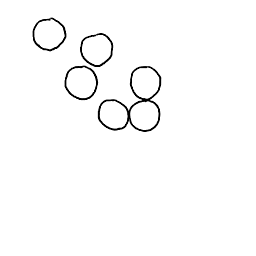
\includegraphics[width = 2cm]{figures/expert-18.png}};
  \node[draw,blue,thick,anchor = west,inner sep=0pt,minimum width = 2cm,minimum height = 2cm,label=below:Canvas: render$(T)$] (canvas) at (0,-4) {};
  \draw[lightgray,ultra thin,step = 0.125] ([xshift = 0.5,yshift = 0.5]canvas.south west) grid ([xshift = -0.5,yshift = -0.5]canvas.north east);
  % draw partial image on canvas
  \draw (0.375cm,-3.25cm) circle (0.125cm);
  \draw (0.625cm,-3.625) circle (0.125cm);
  \draw (0.75cm,-3.375) circle (0.125cm);

  \node[draw,ultra thick,anchor = west,inner sep=0pt,minimum width = 2cm,minimum height = 3cm] (CNN) at (4.5,-2.5) {CNN};
  \node[inner sep = 0pt](tensorProduct) at ([xshift = -1.5cm]CNN.west) {$\bigotimes$};

  \node[rotate = -90,draw,ultra thick,inner sep=0pt,minimum width = 3cm,minimum height = 0.5cm] (features) at ([xshift = 1.5cm]CNN.east) {Image features};

  \node[draw,ultra thick,minimum size = 1cm](c1) at ([xshift = 1.5cm]features.north) {MLP};
  \node(l1) at ([yshift = -2cm]c1.south) {\verb|circle(|};
  \node[draw,ultra thick,minimum size = 1cm](c2) at ([xshift = 1cm]c1.east) {MLP};
  \draw[->,ultra thick,red] (c1.south) -- (l1.north);
  \node(l2) at ([yshift = -2cm]c2.south) {\verb|X=7,|};
  \draw[->,ultra thick,red] (c2.south) -- (l2.north);
  \node[draw,ultra thick,minimum size = 1cm](c3) at ([xshift = 1cm]c2.east) {MLP};
  \node(l3) at ([yshift = -2cm]c3.south) {\verb|Y=12)|};
  \draw[->,ultra thick,red] (c3.south) -- (l3.north);

  
  \draw[->,ultra thick] (features.north) -- (c1.west);
  \draw[->,ultra thick] (features.north) to[out = 45,in = 90] (c2.north);
  \draw[->,ultra thick] (features.north) to[out = 70,in = 90] (c3.north);
  \draw[->,ultra thick] ([xshift = 0.25cm]l1.north) -- (c2.west);
  \draw[->,ultra thick] ([xshift = 0.25cm]l1.north) -- (c3.west);
  \draw[->,ultra thick] ([xshift = 0.25cm]l2.north) -- ([yshift = -0.2cm]c3.west);

  \node(next)[draw,very thick,fit = (l1) (l2) (l3), dashed, label = below:{Next line of code}] {};

  \draw[-{>[scale = 1.5]},very thick,dashed] (next.west) -- ([yshift = -0.2cm]canvas.east) node [midway, below, sloped] (TextNode) {Renderer: \LaTeX~Ti\emph{k}Z};
  
  \draw[->,ultra thick] (canvas.east) -- (tensorProduct.south);%[yshift = -0.5cm]CNN.west);
  \draw[->,ultra thick] (observation.east) -- (tensorProduct.north);%([yshift = 0.5cm]CNN.west);
  \draw[->,ultra thick] (tensorProduct.east)  -- node[fill = white,rotate = 90] {{\tiny $256\times 256\times 2$}}  (CNN.west);
  \draw[->,ultra thick] (CNN.east) -- node[fill = white,rotate = 90] {{\tiny $16\times 16\times 10$}} (features.south);
%  \draw[]
  
%  \node at (canvas.x,canvas.y) {Canvas};
\end{tikzpicture}
\caption{Our neural architecture for inferring the execution trace of a graphics program from its output. \textcolor{blue}{Blue}: network inputs. Black: network operations. \textcolor{red}{Red}: samples from a multinomial. \texttt{Typewriter font}: network outputs. Renders snapped to a $16\times 16$ grid, illustrated in \textcolor{gray}{gray}.}  \label{architecture}
\end{figure}
\begin{table}
\begin{tabular}{ll}\toprule
  \begin{tabular}{l}
    \verb|circle|$(x,y)$
  \end{tabular}& \begin{tabular}{l}
    Circle at $(x,y)$
    \end{tabular}\\
  \begin{tabular}{l}
    \verb|rectangle|$(x_1,y_1,x_2,y_2)$
  \end{tabular}&\begin{tabular}{l}
    Rectangle with corners at $(x_1,y_1)$ \& $(x_2,y_2)$
    \end{tabular}\\
  \begin{tabular}{l}
    \verb|line|$(x_1,y_1,x_2,y_2,$\\
    \hspace{1cm}$\text{arrow}\in\{0,1\},\text{dashed}\in\{0,1\})$
  \end{tabular}&\begin{tabular}{l}
    Line from $(x_1,y_1)$ to  $(x_2,y_2)$,\\\hspace{1cm}optionally with an arrow and/or dashed
    \end{tabular}\\
  \begin{tabular}{l}
    \verb|STOP|
  \end{tabular}&\begin{tabular}{l}
    Finishes execution trace inference
    \end{tabular}
\\  \bottomrule
\end{tabular}
\caption{The deep network in (\ref{architecture}) predicts drawing commands, shown above.}
\label{drawingCommandTable}
\end{table}




This network suffices to ``derender'' synthetic images like those shown in
Figure~\ref{trainingData}.  We can perform a beam search decoding to
recover what the network thinks is the most likely execution trace for
images like these, recovering traces maximizing $\probability_\theta
[T|I]$. But, if the network makes a mistake (predicts an incorrect
line of code), it has no way of recovering from the error.  In order
to derender an image with $n$ objects, it must correctly predict $n$
drawing commands -- so its probability of success will decrease
exponentially in $n$, assuming it has any nonzero chance of making a
mistake.  For added robustness as $n$ becomes large, we treat the
neural network outputs as proposals for a Sequential Monte Carlo (SMC) sampling scheme~\cite{SMCBook}.  For
the SMC sampler, we use pixel-wise distance as a surrogate for a
likelihood function. The SMC sampler is designed to produce samples
from the distribution $\propto L(I|\text{render}(T))
\probability_\theta[T|I]$, where $L(\cdot | \cdot):\text{image}^2\to
\mathcal{R}$ uses the distance between two images as a proxy for a
likelihood.

Figure~\ref{syntheticResults}
compares the neural network with SMC against the neural network by
itself or SMC by itself.  Only the combination of the two passes a
critical test of generalization: when trained on images with $\leq 8$
objects, it successfully parses scenes with many more objects than the
training data.

\begin{figure}\centering
  \begin{minipage}{0.35\textwidth}
    \begin{minipage}[t]{2.2cm}\fbox{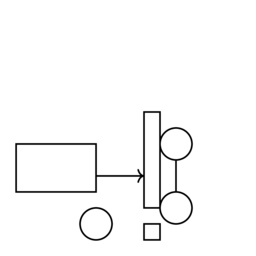
\includegraphics[width=2cm]{figures/randomScene-58-7.png}}\end{minipage}
    \begin{minipage}[t]{2.2cm}\fbox{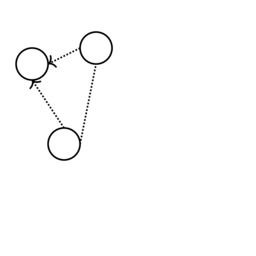
\includegraphics[width=2cm]{figures/randomScene-33-5.png}}\end{minipage}
    \caption{Network is trained to infer execution traces for randomly generated figures like the two shown above. See supplement for details of the training data generation.}\label{trainingData}
  \end{minipage}\hfill
  \begin{minipage}{0.6\textwidth}
    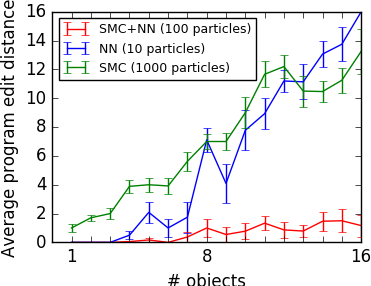
\includegraphics[width = 4cm]{figures/editDistance.png}
    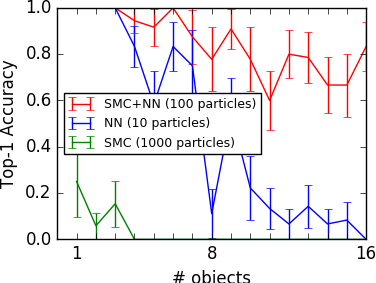
\includegraphics[width = 4cm]{figures/accuracy.png}
      \caption{Using the model to parse latex output. The model is trained on diagrams with up to 8 objects. As shown above it generalizes to scenes with many more objects. Neither the stochastic search nor the neural network are sufficient on their own. \# particles varies by model: we compare the models \emph{with equal runtime} ($\approx 1$ sec/object)}\label{syntheticResults}
    \end{minipage}
  
  \end{figure}

\subsection{Generalizing to hand drawings}
A practical application of our neural network is the automatic conversion of hand drawings into a subset of \LaTeX.
 We train the model
to generalize to hand drawings by introducing noise into the
renderings of the training target images.
We designed this noise process to introduce the kinds of variations found in hand drawings (Figure~\ref{handDrawingExamples}; see supplement for details).
Our neurally-guided SMC procedure
used pixel-wise distance as a surrogate for a likelihood function ($L(\cdot|\cdot)$ in section~\ref{neuralNetworkSection}).
But pixel-wise distance fares poorly on hand drawings, which never exactly match
the model's renders.
So, for hand drawings,
we \emph{learn} a surrogate likelihood function,
$L_{\text{learned}}(\cdot|\cdot)$.
The density $L_{\text{learned}}(\cdot|\cdot)$ is predicted by a convolutional network that we train to predict
the distance between two traces conditioned upon their renderings.
We train our likelihood surrogate to approximate the symmetric difference,
which is  the number of drawing commands by which two traces differ:
\begin{equation}
-\log L_{\text{learned}}(\text{render}(T_1)|\text{render}(T_2))\approx |T_1 - T_2| + |T_2 - T_1|\label{symmetricDistance}
\end{equation}
Intuitively, Eq.~\ref{symmetricDistance} says that
$L_{\text{learned}}(\cdot|\cdot)$ approximates the distance between
the trace we want and the trace we have so far.  Pixel-wise distance
metrics are sensitive to the fine details of how and exactly where
arrows, dashes, and corners are drawn -- but we wish to be invariant
to these details. So, we learn a distance metric over images that
approximates the distance metric in the search space over traces.

We drew 100 figures by hand; see figure~\ref{lotsOfHandDrawings}.
These were drawn reasonably carefully but not perfectly.
Because our model assumes that objects are snapped to a $16\times 16$ grid,
we made the drawings on graph paper.
\begin{figure}\centering
  \begin{minipage}{0.45\textwidth}
  \begin{minipage}[t]{0.3\textwidth}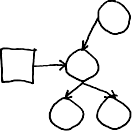
\includegraphics[width = 1.5cm]{figures/expert-60-reduced.png}
    \subcaption{}
  \end{minipage}%
   \begin{minipage}[t]{0.3\textwidth}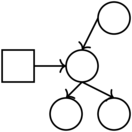
\includegraphics[width = 1.5cm]{figures/60-groundTruth-reduced.png}
    \subcaption{}
  \end{minipage}%
  \begin{minipage}[t]{0.3\textwidth}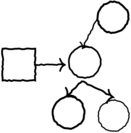
\includegraphics[width = 1.5cm]{figures/60-1-reduced.png}
    \subcaption{}
  \end{minipage}%
    \caption{(a): a hand drawing. (b): Rendering of the trace our model infers for (a). We can generalize to hand drawings like these because we train the model on images corrupted by a noise process designed to resemble the kind of noise introduced by hand drawings - see (c) for a noisy rendering of (b).}\label{handDrawingExamples}
  \end{minipage}\hfill
  \begin{minipage}{0.45\textwidth}
  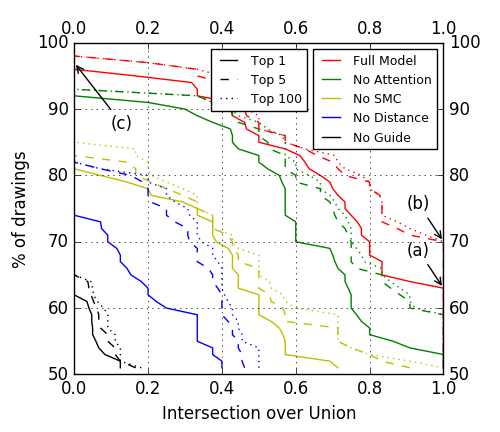
\includegraphics[width = 6cm]{figures/drawingAccuracy.png}
  \caption{How close are the model's outputs to the ground truth on hand drawings, as we consider larger sets of samples (1, 5, 10, 100 samples)?
  Distance to the ground truth trace is measured by the intersection over union of predicted vs. ground truth traces (sets of drawing commands).}\label{drawingIntersectionOverUnion}
    \end{minipage}
\end{figure}


\begin{figure}[H]
  \begin{minipage}[t]{2.25cm}
    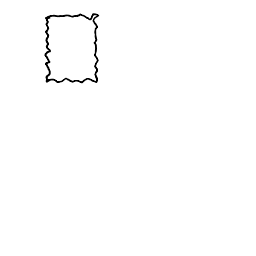
\includegraphics[width = 2cm]{figures/expert-10.png}
    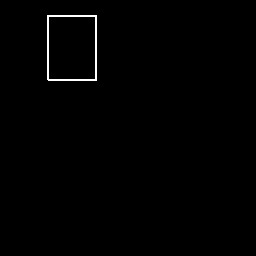
\includegraphics[width = 2cm]{figures/10-parse.png}    
    \subcaption{Noisy input}
  \end{minipage}
  \begin{minipage}[t]{2.25cm}
    \includegraphics[width = 2cm]{figures/expert-21.png}
    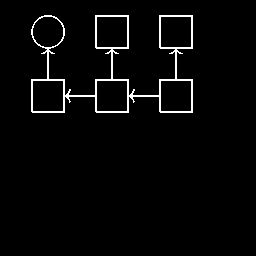
\includegraphics[width = 2cm]{figures/21-parse.png}    
    \subcaption{A graphical model}
  \end{minipage}
  \begin{minipage}[t]{2.25cm}
    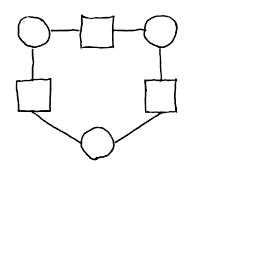
\includegraphics[width = 2cm]{figures/expert-77.png}
    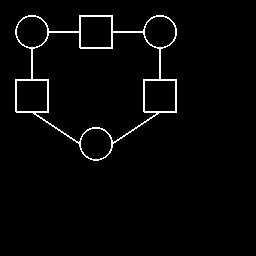
\includegraphics[width = 2cm]{figures/77-parse.png}    
    \subcaption{A figure from a deep learning textbook}
    \end{minipage}
  \begin{minipage}[t]{2.25cm}
    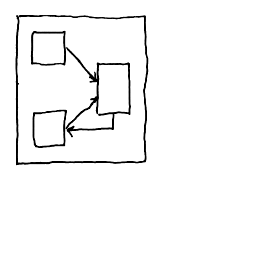
\includegraphics[width = 2cm]{figures/expert-0.png}
    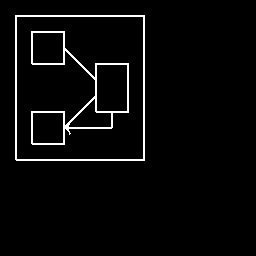
\includegraphics[width = 2cm]{figures/0-parse.png}    
    \subcaption{Near miss}
  \end{minipage}
  \begin{minipage}[t]{2.25cm}
    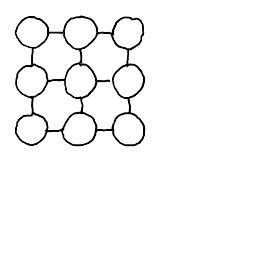
\includegraphics[width = 2cm]{figures/expert-38.png}
    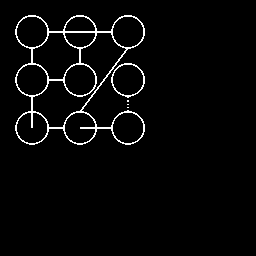
\includegraphics[width = 2cm]{figures/38-parse.png}    
    \subcaption{Failing on a Ising model}
  \end{minipage}
  \begin{minipage}[t]{2.25cm}
    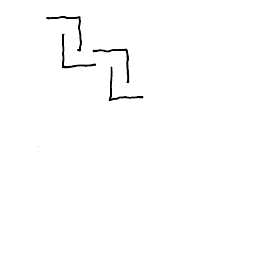
\includegraphics[width = 2cm]{figures/expert-34.png}
    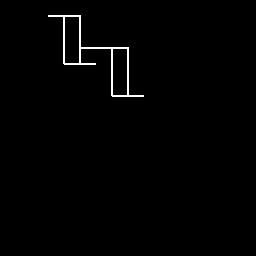
\includegraphics[width = 2cm]{figures/34-parse.png}     
    \subcaption{Illusory contours}
    \end{minipage}
  \caption{Example drawings above model outputs. See also Fig.~\ref{firstPageExamples}. Stochastic search (SMC) can help correct for these errors, as can the program synthesizer (Section~\ref{synthesizerHelpsParsing})}\label{lotsOfHandDrawings}%~\remark{Showing `failure cases' (the last three above) out-of-context seems not great. Perhaps remind people in the caption that stochastic search can help correct some of these issues?}
\end{figure}
For each drawing we annotated a ground truth trace, and evaluated the
model by asking it to sample many candidate traces for each drawing.
For 58\% of the drawings the Top-1 most likely sample exactly matches the
ground truth; as we consider more samples the model encounters traces
that are closer to the ground truth annotation (Fig.~\ref{drawingIntersectionOverUnion}).
Because our current model sometimes makes mistakes on hand drawings,
we envision the current system working as follows:
a user sketches a diagram,
and the system responds by proposing a few candidate interpretations.
The user could then select the one closest to their intention and edit it if necessary.

\section{Synthesizing graphics programs from execution traces}\label{programSynthesisSection}
Although the execution trace of a graphics program describes the parts
of a scene, it fails to encode higher-level features of the image,
such as repeated motifs or symmetries.  A \emph{graphics
  program} better describe structures like these,
and we now take as our goal to synthesize simple graphics programs from
their execution traces.

We constrain the space of allowed programs by writing down a context
free grammar over a space of programs. Although it might be desirable
to synthesize programs in a Turing-complete language such as Lisp or
Python, a more tractable approach is to specify what in the program
languages community is called a Domain Specific Language (DSL)~\cite{polozov2015flashmeta}. Our DSL (Table~\ref{DSL})
encodes prior knowledge of what graphics programs tend to look like.

\begin{table}[H]
  \begin{tabular}{rl}\toprule
  Program$\to$&Command; $\cdots$; Command\\
  Command$\to$&\texttt{circle}(Expression,Expression)\\
  Command$\to$&\texttt{rectangle}(Expression,Expression,Expression,Expression)\\
  Command$\to$&\texttt{line}(Expression,Expression,Expression,Expression,Boolean,Boolean)\\
  Command$\to$&\texttt{for}$(0\leq \text{Var}  < \text{Expression})$\texttt{ \{ if }$(\text{Var} > 0)$\texttt{ \{ }Program\texttt{ \}; }Program\texttt{ \}}\\
  Command$\to$&\texttt{reflect}$(\text{Axis})$\texttt{ \{ }Program\texttt{ \}}\\
  Expression$\to$&$\mathcal{Z}$\texttt{ * }Var\texttt{ + }$\mathcal{Z}$\\
  Var$\to$&A free (unused) variable\\
  $\mathcal{Z}$$\to$&an integer\\
  Axis$\to$&\texttt{X = }$\mathcal{Z}$\\
  Axis$\to$&\texttt{Y = }$\mathcal{Z}$\\\bottomrule
  \end{tabular}
  \caption{Grammar over graphics programs. We allow loops (\texttt{for}) with conditionals (\texttt{if}), vertical/horizontal reflections (\texttt{reflect}), variables (Var) and affine transformations ($\mathcal{Z}$\texttt{ * }Var\texttt{ + }$\mathcal{Z}$).}\label{DSL}
\end{table}

Given the DSL and a trace $T$, we want to recover a program that both evaluates to $T$
and, at the same time, is the ``best'' explanation of $T$.
For example, we might prefer more general programs or, in the spirit of Occam's razor,
prefer shorter programs.
We wrap these intuitions up into a cost function over programs,
and seek the minimum cost program consistent with $T$:
\begin{equation}
  \text{program}(T) = \argmin_{\substack{p\in \text{DSL}\\p \text{ evaluates to } T}} \text{cost}(p)\label{programObjective}
\end{equation}
We define the
cost of a program to be the number of statements it contains, where a
statement is a ``Command'' in Table~\ref{DSL}.
We also penalize using many different numerical constants; see supplement.
%\remark{The flow here is a bit off/backwards. ``We want a program that evaluates to $T$ and also minimizes some measure of program cost''---why do we care about cost? It'd be better to start by making a ``Bayesian Occam's razor'' appeal (e.g. the most compact/general program is the more likely explanation) and then saying that one way to do this is to minimize a cost function which is proportional to program length.}

The constrained optimization problem in
equation~\ref{programObjective} is intractable in general, but there
exist efficient-in-practice tools for finding exact solutions to
program synthesis problems like these. We use the state-of-the-art Sketch
tool~\cite{solar2008program}. Describing Sketch's program synthesis
algorithm is beyond the scope of this paper; see supplement.  At a
high level, Sketch takes as input a space of programs, along with a
specification of the program's behavior and optionally a cost
function.  It translates the synthesis problem into a constraint
satisfaction problem, and then uses a SAT solver to find a
minimum cost program satisfying the specification.  In exchange for
not having any guarantees on how long it will take to find a minimum
cost solution, it comes with the guarantee that it will always find a
globally optimal program.

Why synthesize a graphics program,
if the execution trace already suffices to recover the objects in an image?
Within our domain of hand-drawn figures, graphics program synthesis has several uses:
%\remark{I'm of two minds about how these subsections should be ordered. The current ordering leads with the coolest results, which is nice. But it's a bit...deflating?...to start with such cool results and then end on the somewhat technical point of how the synthesizer can help correct parse errors. An alternative would be to flip the ordering, starting with the technical point and building toward progressively cooler results. This requires a bit more patience on the part of the reader, but the overall narrative flow/payoff feels better. In any case, whatever ordering you pick should be the same order as these applications are mentioned in the abstract.}

\subsection{Correcting errors made by the neural network}\label{synthesizerHelpsParsing}
The program synthesizer can help correct errors from the execution trace proposal network by favoring execution traces which lead to more concise or general programs.
For example, one generally prefers figures with perfectly aligned objects over figures whose parts are slightly misaligned -- and precise alignment lends itself to short programs.
Similarly, figures often have repeated parts,
which the program synthesizer might be able to model as a loop or reflectional symmetry.
So, in considering several candidate traces proposed by the neural network,
we might prefer traces whose best programs have desirable features such being short or having iterated structures.

Concretely, we implemented the following scheme: the neurally guided sampling scheme of section~\ref{neuralNetworkSection} for image $I$ samples candidate traces $\mathcal{F}(I)$.
Instead of predicting the most likely trace in $\mathcal{F}(I)$ according to the neural network,
we can take into account the programs that best explain the traces. 
Writing $\hat{T}(I)$ for the trace the model predicts for image $I$,
\begin{equation}
\hat{T}(I) = \argmax_{T\in \mathcal{F}(I)} L_{\text{learned}}(I | \text{render}(T)) \times\probability_{\beta} [ \text{program}(T)] 
\end{equation}
where $\probability_{\beta} [\cdot]$ is a prior probability
distribution over programs parameterized by $\beta$.
This is equivalent to doing
MAP inference in a generative model where the program is first drawn
from $\probability_{\beta} [\cdot]$, then the program is executed deterministically,
and then we observe a noisy version of the program's output, where $L$
is the noise model.

Given a corpus of graphics program synthesis problems with annotated ground truth traces (i.e. $(I,T)$ pairs),
we find a maximum likelihood estimate of $\beta$:
\begin{equation}
  \beta^* = \argmax_{\beta} \expect \left[ \log \frac{\probability_{\beta} [\text{program}(T)]\times L_{\text{learned}}(I|\text{render}(T))}{\sum_{T'\in \mathcal{F}(I)} \probability_{\beta} [\text{program}(T')]\times L_{\text{learned}}(I|\text{render}(T'))} \right]
\end{equation}
where the expectation is taken both over the model predictions and the
$(I,T)$ pairs in the training corpus.  We define $\probability_{\beta}
[\cdot]$ to be a log linear distribution $\propto \exp
(\beta\cdot \phi(\text{program}))$, where $\phi(\cdot)$ is a feature
extractor for programs.  We extract a few basic features of a
program, such as its size and how many loops it has, and use these
features to help predict whether a trace is the correct explanation
for an image.

We synthesized programs for the top five traces
output by the deep network.  Learning this prior over programs can
help correct mistakes made by the neural network, and also
occasionally introduces mistakes of its own; see
Fig.~\ref{exampleOfProgramCorrectingMistake} for a representative
example of the kinds of corrections that it makes. On the whole
modestly improves our Top-1 accuracy from 58\% to 60\%.  Recall that
from Fig.~\ref{drawingIntersectionOverUnion} that the best improvement
in accuracy we could possibly get is 63\% by looking at the top 5 traces.
\begin{wrapfigure}{R}{5.5cm}
  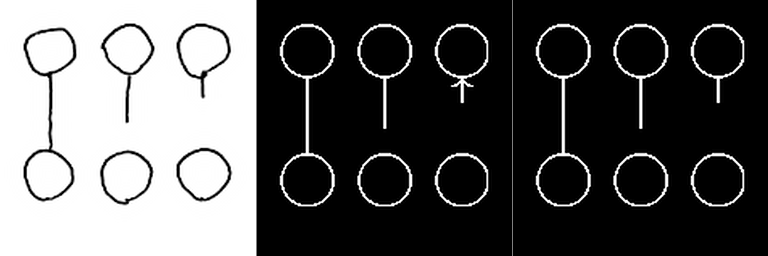
\includegraphics[width = 5cm]{figures/programSuccess7.png}
  \caption{Left: hand drawing. Center: interpretation favored by the deep network. Right: interpretation favored after learning a prior over programs.}\label{exampleOfProgramCorrectingMistake}
  \end{wrapfigure}

\subsection{Modeling similarity between drawings}
Modeling an image using a program opens up new ways of measuring similarity between drawings.
For example, we might say that two drawings are similar if they both contain repetitions of length 4,
or if they share the same reflectional symmetry,
or if they are both organized according to a grid-like structure.

We measure the similarity between two drawings by extracting features
of the best programs that describe them.  Here the features we use are
just counts of the number of times that different components in the
DSL were used (Table~\ref{DSL}).  We project these features down to a
2-dimensional subspace using nonnegative matrix factorization
(NMF:~\cite{lee1999learning}); see Fig.\ref{NMF}.  One could use many
alternative similarity metrics between drawings which would capture pixel-level or object-level similarities while missing high-level geometric similarities.
For example, we can use our learned distance metric between execution traces, $L_{\text{learned}}(\cdot|\cdot)$.
Projecting these distances to a 2-dimensional subspace using multidimensional scaling (MDS:~\cite{cox2008multidimensional}) reveals similarities between the objects in the drawings,
while missing similarities at the level of the program.
\begin{figure}
  \begin{minipage}{0.45\textwidth}
    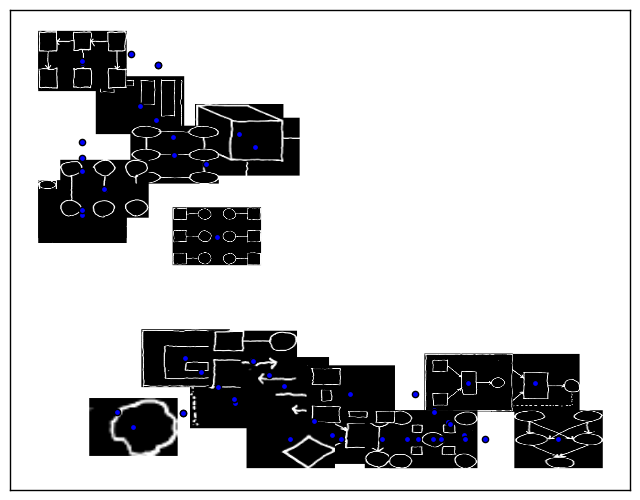
\includegraphics[width = 2in]{figures/NMF.png}
    \caption{NMF on features of the programs that were synthesized for each image. Horizontal component roughly corresponds to ``symmetry'' while vertical component roughly corresponds to ``loopyness'', with images on the diagonal having both of these.}    \label{NMF}
  \end{minipage}\hfill
  \begin{minipage}{0.45\textwidth}
    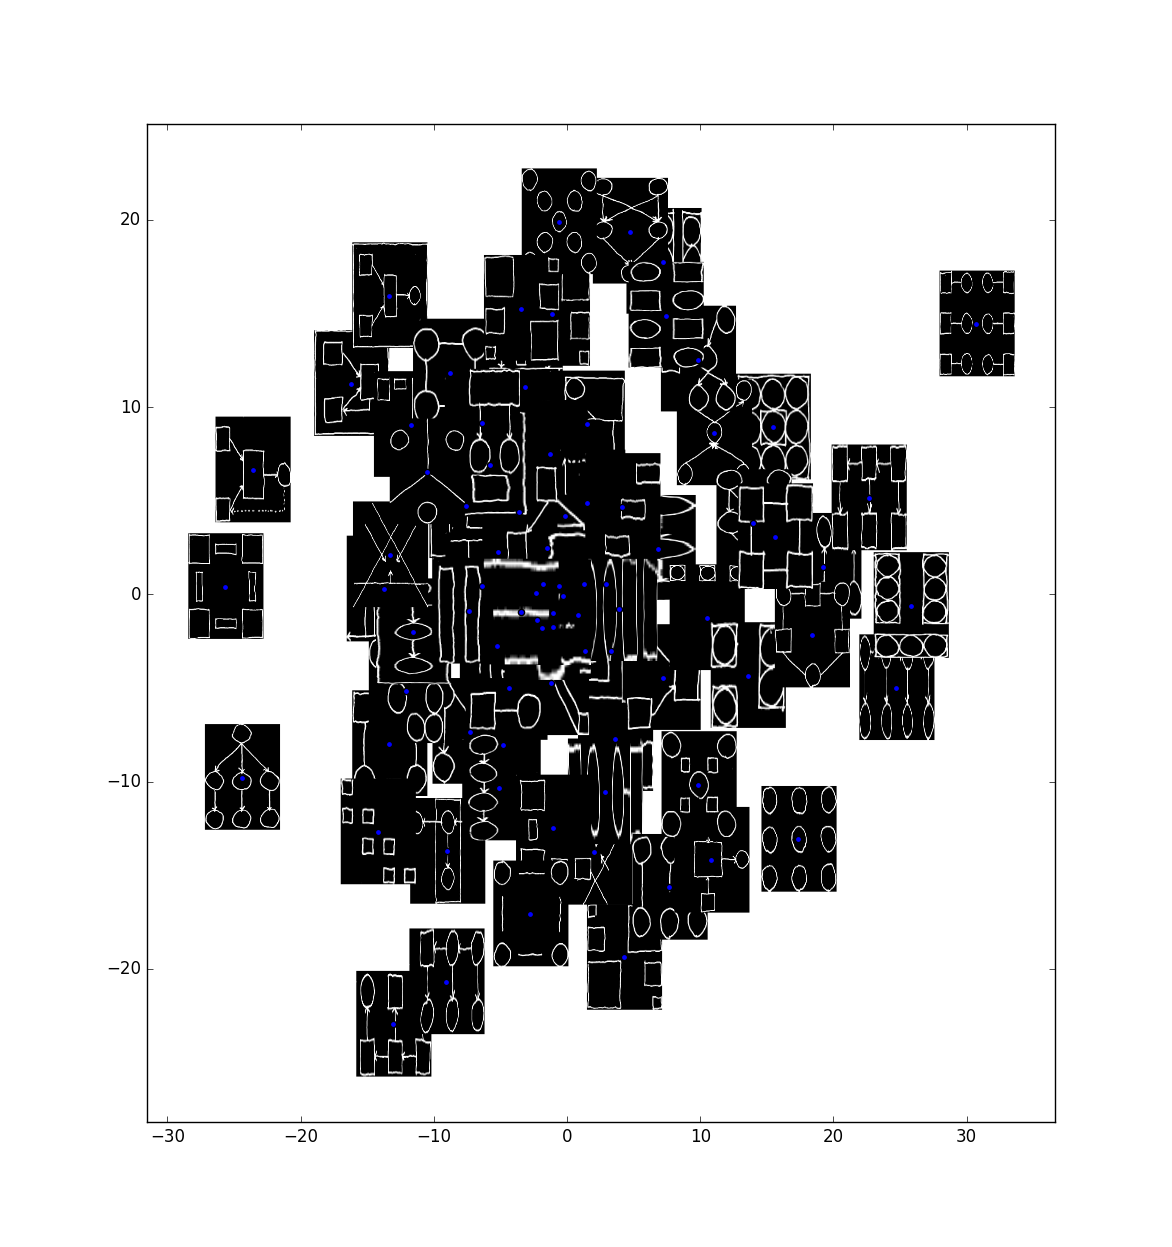
\includegraphics[width = 2in]{figures/imageSimilarity.png} 
    \caption{MDS on drawings using the learned distance metric, $L_{\text{learned}}(\cdot|\cdot)$. Drawings with similar looking parts in similar locations are clustered together.}
  \end{minipage}
\end{figure}

\subsection{Extrapolating figures}
Having access to the source code of a graphics program facilitates coherent, high-level edits to the figure generated by that program. 
For example,
we can change all of the circles to squares or make all of the lines be dashed.
We can also \textbf{extrapolate} figures
by increasing the number of times that loops are executed.
Extrapolating repetitive visuals patterns comes naturally to humans,
and building this ability into an application is practical:
imagine hand drawing a repetitive graphical model structure
and having our system automatically induce and extend the pattern.
Fig.~\ref{extrapolationFigure} shows extrapolations of programs synthesized from ground truth traces;
see supplement for our full set of extrapolations.

\begin{figure}
  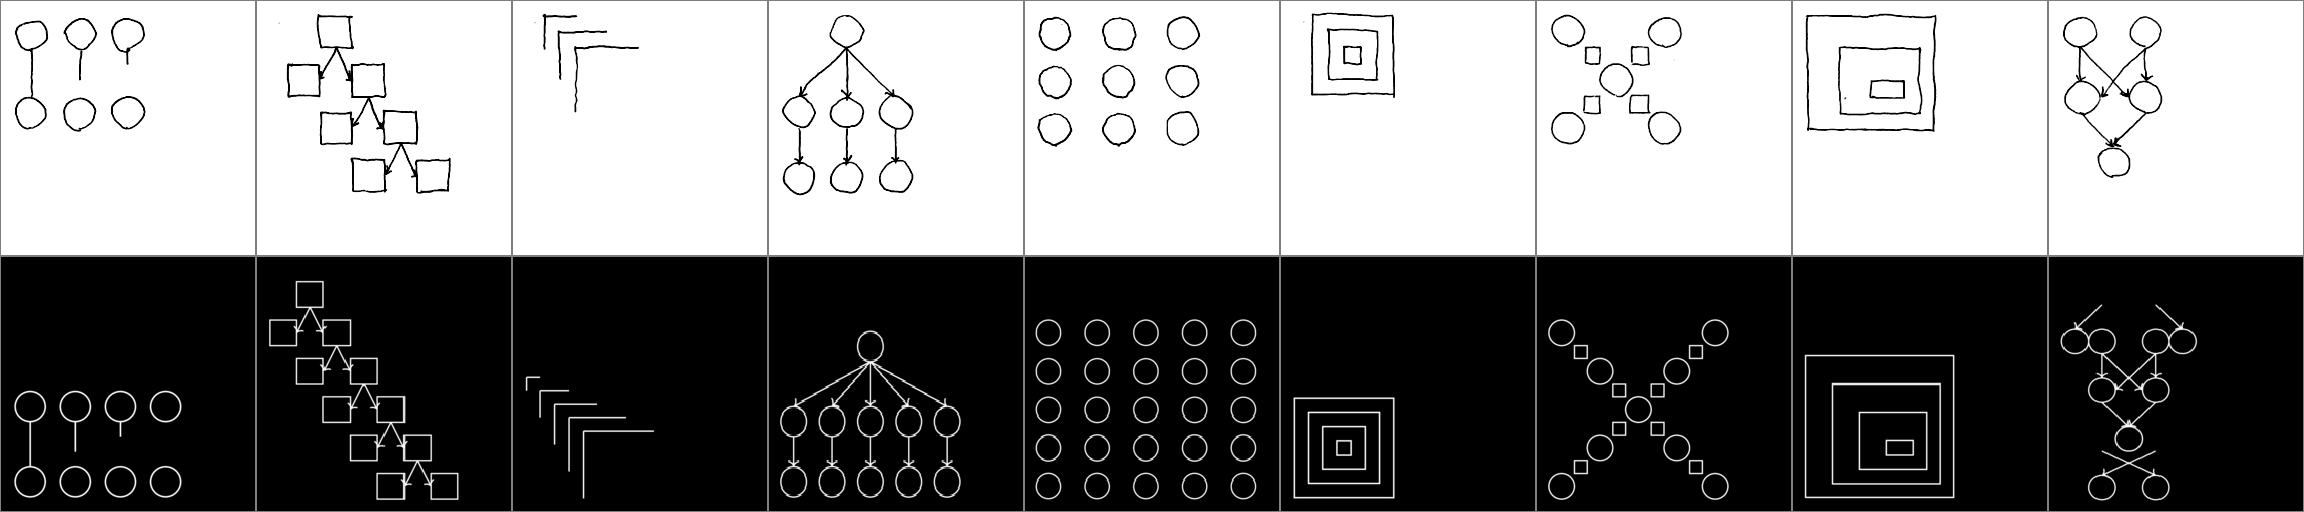
\includegraphics[width = \textwidth]{figures/extrapolationMatrix.png} 
  \caption{Top: hand drawings. Bottom: extrapolations produced by
running loops for extra iterations. Rightmost pair is an illustrative failure case.}\label{extrapolationFigure}
  \end{figure}
%
            \begin{tabular}{ll}
    \includegraphics[width = 5cm]{../TikZ/drawings/expert-17.png}&
    \includegraphics[width = 5cm]{../TikZ/extrapolations/expert-17-extrapolation.png}
    \end{tabular}        
            \\

            \begin{tabular}{ll}
    \includegraphics[width = 5cm]{../TikZ/drawings/expert-21.png}&
    \includegraphics[width = 5cm]{../TikZ/extrapolations/expert-21-extrapolation.png}
    \end{tabular}        
            \\

            \begin{tabular}{ll}
    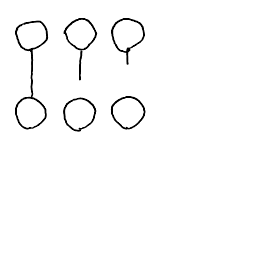
\includegraphics[width = 5cm]{../TikZ/drawings/expert-7.png}&
    \includegraphics[width = 5cm]{../TikZ/extrapolations/expert-7-extrapolation.png}
    \end{tabular}        
            \\

            \begin{tabular}{ll}
    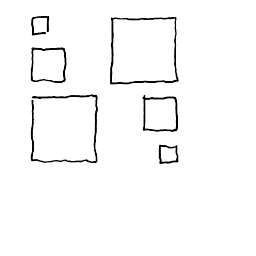
\includegraphics[width = 5cm]{../TikZ/drawings/expert-36.png}&
    \includegraphics[width = 5cm]{../TikZ/extrapolations/expert-36-extrapolation.png}
    \end{tabular}        
            \\

            \begin{tabular}{ll}
    \includegraphics[width = 5cm]{../TikZ/drawings/expert-58.png}&
    \includegraphics[width = 5cm]{../TikZ/extrapolations/expert-58-extrapolation.png}
    \end{tabular}        
            \\

            \begin{tabular}{ll}
    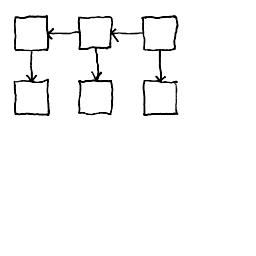
\includegraphics[width = 5cm]{../TikZ/drawings/expert-22.png}&
    \includegraphics[width = 5cm]{../TikZ/extrapolations/expert-22-extrapolation.png}
    \end{tabular}        
            \\

            \begin{tabular}{ll}
    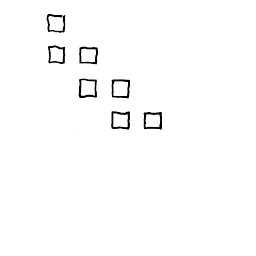
\includegraphics[width = 5cm]{../TikZ/drawings/expert-14.png}&
    \includegraphics[width = 5cm]{../TikZ/extrapolations/expert-14-extrapolation.png}
    \end{tabular}        
            \\

            \begin{tabular}{ll}
    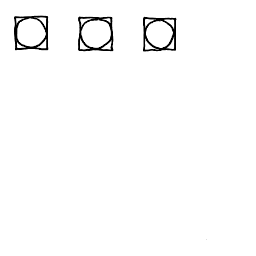
\includegraphics[width = 5cm]{../TikZ/drawings/expert-68.png}&
    \includegraphics[width = 5cm]{../TikZ/extrapolations/expert-68-extrapolation.png}
    \end{tabular}        
            \\

            \begin{tabular}{ll}
    \includegraphics[width = 5cm]{../TikZ/drawings/expert-12.png}&
    \includegraphics[width = 5cm]{../TikZ/extrapolations/expert-12-extrapolation.png}
    \end{tabular}        
            \\

            \begin{tabular}{ll}
    \includegraphics[width = 5cm]{../TikZ/drawings/expert-35.png}&
    \includegraphics[width = 5cm]{../TikZ/extrapolations/expert-35-extrapolation.png}
    \end{tabular}        
            \\

            \begin{tabular}{ll}
    \includegraphics[width = 5cm]{../TikZ/drawings/expert-31.png}&
    \includegraphics[width = 5cm]{../TikZ/extrapolations/expert-31-extrapolation.png}
    \end{tabular}        
            \\

            \begin{tabular}{ll}
    \includegraphics[width = 5cm]{../TikZ/drawings/expert-37.png}&
    \includegraphics[width = 5cm]{../TikZ/extrapolations/expert-37-extrapolation.png}
    \end{tabular}        
            \\

            \begin{tabular}{ll}
    \includegraphics[width = 5cm]{../TikZ/drawings/expert-29.png}&
    \includegraphics[width = 5cm]{../TikZ/extrapolations/expert-29-extrapolation.png}
    \end{tabular}        
            \\

            \begin{tabular}{ll}
    \includegraphics[width = 5cm]{../TikZ/drawings/expert-57.png}&
    \includegraphics[width = 5cm]{../TikZ/extrapolations/expert-57-extrapolation.png}
    \end{tabular}        
            \\

            \begin{tabular}{ll}
    \includegraphics[width = 5cm]{../TikZ/drawings/expert-23.png}&
    \includegraphics[width = 5cm]{../TikZ/extrapolations/expert-23-extrapolation.png}
    \end{tabular}        
            \\

            \begin{tabular}{ll}
    \includegraphics[width = 5cm]{../TikZ/drawings/expert-60.png}&
    \includegraphics[width = 5cm]{../TikZ/extrapolations/expert-60-extrapolation.png}
    \end{tabular}        
            \\

            \begin{tabular}{ll}
    \includegraphics[width = 5cm]{../TikZ/drawings/expert-16.png}&
    \includegraphics[width = 5cm]{../TikZ/extrapolations/expert-16-extrapolation.png}
    \end{tabular}        
            \\

            \begin{tabular}{ll}
    \includegraphics[width = 5cm]{../TikZ/drawings/expert-5.png}&
    \includegraphics[width = 5cm]{../TikZ/extrapolations/expert-5-extrapolation.png}
    \end{tabular}        
            \\

            \begin{tabular}{ll}
    \includegraphics[width = 5cm]{../TikZ/drawings/expert-50.png}&
    \includegraphics[width = 5cm]{../TikZ/extrapolations/expert-50-extrapolation.png}
    \end{tabular}        
            \\

            \begin{tabular}{ll}
    \includegraphics[width = 5cm]{../TikZ/drawings/expert-6.png}&
    \includegraphics[width = 5cm]{../TikZ/extrapolations/expert-6-extrapolation.png}
    \end{tabular}        
            



% \remark{Seems like you're still fleshing this part out, but I'll give my feedback anyway: (1) This subsection could really use a motivational introduction, e.g. ``The program synthesizer can help correct errors/bad proposals from the neural network by favoring execution traces which lead to more concise/general programs.'' (2) The image likelihood function should probably be introduced sooner, when you talk about SMC/beam search. (3) Where does $\theta$ come from? Is it set by hand? Learned? (4) How does Equation 4 get used? Is this a modification to the beam search objective / SMC posterior? If so, it'd be great to have set up the version without it in an earlier section, and then be able to refer to this as a small modification of the previous equation.}


\section{Conclusion}

We have presented a system for inferring graphics programs which generate \LaTeX-style figures from hand-drawn images. The system uses a combination of deep neural networks and stochastic search to parse drawings into symbolic execution traces; it then feeds these traces to a general-purpose program synthesis engine to infer a structured graphics program. We evaluated our model's performance at parsing novel images, and we demonstrated its ability to extrapolate from provided drawings and to organize them according to high-level geometric features.

There are many directions for future work. In the parsing phase, the proposal network currently samples positional variables on a discrete grid. More general types of drawings could be supported by instead sampling from continuous distributions, e.g. using Mixture Density Networks~\cite{MDN}. The proposal network also currently handles only a very small subset of \LaTeX drawing commands, though there is no reason that it could not be extended to handle more with a higher-capacity network. Exploring more sophisticated network architectures, including ones that utilize attention, could also help correct some of the errors the network makes.
In the synthesis phase, a more expressive DSL---including subroutines, recursion, and symmetry groups beyond reflections---would allow the system to effectively model a wider variety of graphical phenomena. The synthesizer itself could also be the subject of future work: the system currently uses the general-purpose Sketch synthesizer, which can take minutes to hours to run, whereas program synthesizers which are custom-built for special problem domains can run much faster or even interactively~\cite{le2014flashextract}.

In the not-too-distant future, we believe it should be possible to produce professional-looking figures just by drawing them and then letting an artificially-intelligent agent write the corresponding code.
More generally, we believe that the two-phase system we have proposed---parsing into execution traces, then searching for a low-cost symbolic program which generates those traces---may be a useful paradigm for other domains in which agents must programmatically reason about noisy perceptual input.



%
            \begin{tabular}{lll}
    \includegraphics[width = 5cm]{../TikZ/drawings/expert-0.png}&
            \includegraphics[width = 5cm]{../TikZ/drawings/expert-0-parses/0.png}&
    
        \begin{minipage}{10cm}
        \begin{verbatim}
line(6,2,6,3,
arrow = False,solid = True);
line(6,2,3,2,
arrow = True,solid = True);
reflect(reflect(y = 9)){
line(3,2,5,4,
arrow = True,solid = True);
rectangle(0,0,8,9);
rectangle(5,3,7,6);
rectangle(1,1,3,3)
}
        \end{verbatim}
\end{minipage}

    \end{tabular}        
            \\

            \begin{tabular}{lll}
    \includegraphics[width = 5cm]{../TikZ/drawings/expert-1.png}&
            \includegraphics[width = 5cm]{../TikZ/drawings/expert-1-parses/0.png}&
    
        \begin{minipage}{10cm}
        \begin{verbatim}
Solver timeout
        \end{verbatim}
\end{minipage}

    \end{tabular}        
            \\

            \begin{tabular}{lll}
    \includegraphics[width = 5cm]{../TikZ/drawings/expert-2.png}&
            \includegraphics[width = 5cm]{../TikZ/drawings/expert-2-parses/0.png}&
    
        \begin{minipage}{10cm}
        \begin{verbatim}
rectangle(4,2,6,5);
reflect(reflect(y = 7)){
line(2,6,4,4,
arrow = True,solid = True);
rectangle(0,0,2,2)
}
        \end{verbatim}
\end{minipage}

    \end{tabular}        
            \\

            \begin{tabular}{lll}
    \includegraphics[width = 5cm]{../TikZ/drawings/expert-3.png}&
            \includegraphics[width = 5cm]{../TikZ/drawings/expert-3-parses/0.png}&
    
        \begin{minipage}{10cm}
        \begin{verbatim}
circle(10,5);
line(7,5,9,5,
arrow = True,solid = True);
rectangle(5,3,7,7);
rectangle(0,0,12,10);
reflect(reflect(y = 10)){
line(3,8,5,6,
arrow = True,solid = True);
rectangle(1,7,3,9)
}
        \end{verbatim}
\end{minipage}

    \end{tabular}        
            \\

            \begin{tabular}{lll}
    \includegraphics[width = 5cm]{../TikZ/drawings/expert-4.png}&
            \includegraphics[width = 5cm]{../TikZ/drawings/expert-4-parses/0.png}&
    
        \begin{minipage}{10cm}
        \begin{verbatim}
circle(10,4);
line(10,1,2,1,
arrow = True,solid = False);
line(10,1,10,3,
arrow = False,solid = False);
line(7,4,9,4,
arrow = True,solid = True);
reflect(reflect(y = 8)){
line(2,7,4,5,
arrow = True,solid = True);
rectangle(4,2,7,6);
rectangle(0,6,2,8)
}
        \end{verbatim}
\end{minipage}

    \end{tabular}        
            \\

            \begin{tabular}{lll}
    \includegraphics[width = 5cm]{../TikZ/drawings/expert-5.png}&
            \includegraphics[width = 5cm]{../TikZ/drawings/expert-5-parses/0.png}&
    
        \begin{minipage}{10cm}
        \begin{verbatim}
Solver timeout
        \end{verbatim}
\end{minipage}

    \end{tabular}        
            \\

            \begin{tabular}{lll}
    \includegraphics[width = 5cm]{../TikZ/drawings/expert-6.png}&
            \includegraphics[width = 5cm]{../TikZ/drawings/expert-6-parses/0.png}&
    
        \begin{minipage}{10cm}
        \begin{verbatim}
line(0,1,2,0,
arrow = False,solid = True);
for (i < 3){
if (i > 0){
line(3*i + -3,4,3*i + -1,3,
arrow = False,solid = True);
line(0,3*i + -2,3*i + -3,4,
arrow = False,solid = True)
}
rectangle(2,0,5,3)
}
        \end{verbatim}
\end{minipage}

    \end{tabular}        
            \\

            \begin{tabular}{lll}
    \includegraphics[width = 5cm]{../TikZ/drawings/expert-7.png}&
            \includegraphics[width = 5cm]{../TikZ/drawings/expert-7-parses/0.png}&
    
        \begin{minipage}{10cm}
        \begin{verbatim}
for (i < 3){
circle(-3*i + 7,1);
circle(-3*i + 7,6);
line(-3*i + 7,-1*i + 4,-3*i + 7,5,
arrow = False,solid = True)
}
        \end{verbatim}
\end{minipage}

    \end{tabular}        
            \\

            \begin{tabular}{lll}
    \includegraphics[width = 5cm]{../TikZ/drawings/expert-8.png}&
            \includegraphics[width = 5cm]{../TikZ/drawings/expert-8-parses/0.png}&
    
        \begin{minipage}{10cm}
        \begin{verbatim}
line(0,0,0,4,
arrow = False,solid = True)
        \end{verbatim}
\end{minipage}

    \end{tabular}        
            \\

            \begin{tabular}{lll}
    \includegraphics[width = 5cm]{../TikZ/drawings/expert-9.png}&
            \includegraphics[width = 5cm]{../TikZ/drawings/expert-9-parses/0.png}&
    
        \begin{minipage}{10cm}
        \begin{verbatim}
line(6,0,0,0,
arrow = True,solid = True)
        \end{verbatim}
\end{minipage}

    \end{tabular}        
            \\

            \begin{tabular}{lll}
    \includegraphics[width = 5cm]{../TikZ/drawings/expert-10.png}&
            \includegraphics[width = 5cm]{../TikZ/drawings/expert-10-parses/0.png}&
    
        \begin{minipage}{10cm}
        \begin{verbatim}
rectangle(0,0,3,4)
        \end{verbatim}
\end{minipage}

    \end{tabular}        
            \\

            \begin{tabular}{lll}
    \includegraphics[width = 5cm]{../TikZ/drawings/expert-11.png}&
            \includegraphics[width = 5cm]{../TikZ/drawings/expert-11-parses/0.png}&
    
        \begin{minipage}{10cm}
        \begin{verbatim}
circle(1,1)
        \end{verbatim}
\end{minipage}

    \end{tabular}        
            \\

            \begin{tabular}{lll}
    \includegraphics[width = 5cm]{../TikZ/drawings/expert-12.png}&
            \includegraphics[width = 5cm]{../TikZ/drawings/expert-12-parses/0.png}&
    
        \begin{minipage}{10cm}
        \begin{verbatim}
line(2,6,5,6,
arrow = False,solid = True);
reflect(reflect(x = 7)){
circle(6,1);
line(2,1,5,1,
arrow = False,solid = True);
line(1,2,1,5,
arrow = False,solid = True);
rectangle(5,5,7,7)
}
        \end{verbatim}
\end{minipage}

    \end{tabular}        
            \\

            \begin{tabular}{lll}
    \includegraphics[width = 5cm]{../TikZ/drawings/expert-13.png}&
            \includegraphics[width = 5cm]{../TikZ/drawings/expert-13-parses/0.png}&
    
        \begin{minipage}{10cm}
        \begin{verbatim}
line(2,1,4,1,
arrow = True,solid = True);
line(3,2,1,2,
arrow = True,solid = True);
line(5,0,3,0,
arrow = True,solid = True);
line(0,3,2,3,
arrow = True,solid = True)
        \end{verbatim}
\end{minipage}

    \end{tabular}        
            \\

            \begin{tabular}{lll}
    \includegraphics[width = 5cm]{../TikZ/drawings/expert-14.png}&
            \includegraphics[width = 5cm]{../TikZ/drawings/expert-14-parses/0.png}&
    
        \begin{minipage}{10cm}
        \begin{verbatim}
for (i < 4){
if (i > 0){
rectangle(-2*i + 6,2*i + -2,-2*i + 7,2*i + -1)
}
rectangle(-2*i + 6,2*i,-2*i + 7,2*i + 1)
}
        \end{verbatim}
\end{minipage}

    \end{tabular}        
            \\

            \begin{tabular}{lll}
    \includegraphics[width = 5cm]{../TikZ/drawings/expert-15.png}&
            \includegraphics[width = 5cm]{../TikZ/drawings/expert-15-parses/0.png}&
    
        \begin{minipage}{10cm}
        \begin{verbatim}
line(0,3,2,3,
arrow = False,solid = False);
line(2,1,4,1,
arrow = False,solid = False);
line(1,2,3,2,
arrow = False,solid = True);
line(3,0,5,0,
arrow = False,solid = True)
        \end{verbatim}
\end{minipage}

    \end{tabular}        
            \\

            \begin{tabular}{lll}
    \includegraphics[width = 5cm]{../TikZ/drawings/expert-16.png}&
            \includegraphics[width = 5cm]{../TikZ/drawings/expert-16-parses/0.png}&
    
        \begin{minipage}{10cm}
        \begin{verbatim}
for (i < 4){
if (i > 0){
circle(-2*i + 7,3*i + -2);
line(-2*i + 9,3*i,-2*i + 10,3*i + -2,
arrow = False,solid = True);
line(-2*i + 8,3*i + -2,-2*i + 9,3*i,
arrow = False,solid = True)
}
circle(-2*i + 9,3*i + 1)
}
        \end{verbatim}
\end{minipage}

    \end{tabular}        
            \\

            \begin{tabular}{lll}
    \includegraphics[width = 5cm]{../TikZ/drawings/expert-17.png}&
            \includegraphics[width = 5cm]{../TikZ/drawings/expert-17-parses/0.png}&
    
        \begin{minipage}{10cm}
        \begin{verbatim}
for (i < 4){
if (i > 0){
line(2*i + 1,-3*i + 12,2*i,-3*i + 10,
arrow = True,solid = True);
line(2*i + 1,-3*i + 12,2*i + 2,-3*i + 10,
arrow = True,solid = True);
rectangle(2*i + -2,-3*i + 9,2*i,-3*i + 11)
}
rectangle(2*i + 2,-3*i + 9,2*i + 4,-3*i + 11)
}
        \end{verbatim}
\end{minipage}

    \end{tabular}        
            \\

            \begin{tabular}{lll}
    \includegraphics[width = 5cm]{../TikZ/drawings/expert-18.png}&
            \includegraphics[width = 5cm]{../TikZ/drawings/expert-18-parses/0.png}&
    
        \begin{minipage}{10cm}
        \begin{verbatim}
circle(5,1);
for (i < 3){
if (i > 0){
circle(7,2*i + -1);
circle(i + 2,2*i + 1)
}
circle(1,6)
}
        \end{verbatim}
\end{minipage}

    \end{tabular}        
            \\

            \begin{tabular}{lll}
    \includegraphics[width = 5cm]{../TikZ/drawings/expert-19.png}&
            \includegraphics[width = 5cm]{../TikZ/drawings/expert-19-parses/0.png}&
    
        \begin{minipage}{10cm}
        \begin{verbatim}
line(4,4,2,2,
arrow = True,solid = True);
rectangle(3,4,5,6);
rectangle(0,0,2,2)
        \end{verbatim}
\end{minipage}

    \end{tabular}        
            \\

            \begin{tabular}{lll}
    \includegraphics[width = 5cm]{../TikZ/drawings/expert-20.png}&
            \includegraphics[width = 5cm]{../TikZ/drawings/expert-20-parses/0.png}&
    
        \begin{minipage}{10cm}
        \begin{verbatim}
rectangle(0,4,2,6);
for (i < 3){
if (i > 0){
line(-4*i + 12,5,-4*i + 10,5,
arrow = True,solid = True);
for (j < i + 1){
circle(-4*j + 9,-4*i + 9)
}
}
line(-4*i + 9,4,-4*i + 9,2,
arrow = True,solid = True)
}
        \end{verbatim}
\end{minipage}

    \end{tabular}        
            \\

            \begin{tabular}{lll}
    \includegraphics[width = 5cm]{../TikZ/drawings/expert-21.png}&
            \includegraphics[width = 5cm]{../TikZ/drawings/expert-21-parses/0.png}&
    
        \begin{minipage}{10cm}
        \begin{verbatim}
Solver timeout
        \end{verbatim}
\end{minipage}

    \end{tabular}        
            \\

            \begin{tabular}{lll}
    \includegraphics[width = 5cm]{../TikZ/drawings/expert-22.png}&
            \includegraphics[width = 5cm]{../TikZ/drawings/expert-22-parses/0.png}&
    
        \begin{minipage}{10cm}
        \begin{verbatim}
for (i < 3){
line(-4*i + 9,4,-4*i + 9,2,
arrow = True,solid = True);
for (j < 2){
line(-4*j + 8,5,-4*j + 6,5,
arrow = True,solid = True);
rectangle(-4*i + 8,4*j,-4*i + 10,4*j + 2)
}
}
        \end{verbatim}
\end{minipage}

    \end{tabular}        
            \\

            \begin{tabular}{lll}
    \includegraphics[width = 5cm]{../TikZ/drawings/expert-23.png}&
            \includegraphics[width = 5cm]{../TikZ/drawings/expert-23-parses/0.png}&
    
        \begin{minipage}{10cm}
        \begin{verbatim}
for (i < 3){
if (i > 0){
line(-4*i + 12,1,-4*i + 10,1,
arrow = True,solid = True)
}
circle(-4*i + 9,1);
circle(-4*i + 9,5);
line(-4*i + 9,2,-4*i + 9,4,
arrow = True,solid = True)
}
        \end{verbatim}
\end{minipage}

    \end{tabular}        
            \\

            \begin{tabular}{lll}
    \includegraphics[width = 5cm]{../TikZ/drawings/expert-24.png}&
            \includegraphics[width = 5cm]{../TikZ/drawings/expert-24-parses/0.png}&
    
        \begin{minipage}{10cm}
        \begin{verbatim}
reflect(reflect(x = 6)){
for (i < 3){
if (i > 0){
line(-2*i + 7,-4*i + 11,-2*i + 7,-4*i + 10,
arrow = True,solid = True);
rectangle(0,-4*i + 11,6,-3*i + 12)
}
rectangle(2,0,4,2)
}
}
        \end{verbatim}
\end{minipage}

    \end{tabular}        
            \\

            \begin{tabular}{lll}
    \includegraphics[width = 5cm]{../TikZ/drawings/expert-25.png}&
            \includegraphics[width = 5cm]{../TikZ/drawings/expert-25-parses/0.png}&
    
        \begin{minipage}{10cm}
        \begin{verbatim}
for (i < 3){
if (i > 0){
line(3*i,1,3*i + -1,1,
arrow = True,solid = True)
}
rectangle(3*i,0,3*i + 2,2)
}
        \end{verbatim}
\end{minipage}

    \end{tabular}        
            \\

            \begin{tabular}{lll}
    \includegraphics[width = 5cm]{../TikZ/drawings/expert-26.png}&
            \includegraphics[width = 5cm]{../TikZ/drawings/expert-26-parses/0.png}&
    
        \begin{minipage}{10cm}
        \begin{verbatim}
line(1,3,1,4,
arrow = False,solid = True);
for (i < 3){
if (i > 0){
line(1,-5*i + 13,1,-4*i + 10,
arrow = True,solid = True)
}
circle(1,-4*i + 9)
}
        \end{verbatim}
\end{minipage}

    \end{tabular}        
            \\

            \begin{tabular}{lll}
    \includegraphics[width = 5cm]{../TikZ/drawings/expert-27.png}&
            \includegraphics[width = 5cm]{../TikZ/drawings/expert-27-parses/0.png}&
    
        \begin{minipage}{10cm}
        \begin{verbatim}
reflect(reflect(x = 2)){
line(0,1,1,2,
arrow = False,solid = True);
line(1,0,2,1,
arrow = False,solid = True)
}
        \end{verbatim}
\end{minipage}

    \end{tabular}        
            \\

            \begin{tabular}{lll}
    \includegraphics[width = 5cm]{../TikZ/drawings/expert-28.png}&
            \includegraphics[width = 5cm]{../TikZ/drawings/expert-28-parses/0.png}&
    
        \begin{minipage}{10cm}
        \begin{verbatim}
line(0,0,0,2,
arrow = False,solid = True);
line(0,2,2,2,
arrow = False,solid = True)
        \end{verbatim}
\end{minipage}

    \end{tabular}        
            \\

            \begin{tabular}{lll}
    \includegraphics[width = 5cm]{../TikZ/drawings/expert-29.png}&
            \includegraphics[width = 5cm]{../TikZ/drawings/expert-29-parses/0.png}&
    
        \begin{minipage}{10cm}
        \begin{verbatim}
for (i < 3){
line(i,-1*i + 6,2*i + 2,-1*i + 6,
arrow = False,solid = True);
line(i,-2*i + 4,i,-1*i + 6,
arrow = False,solid = True)
}
        \end{verbatim}
\end{minipage}

    \end{tabular}        
            \\

            \begin{tabular}{lll}
    \includegraphics[width = 5cm]{../TikZ/drawings/expert-30.png}&
            \includegraphics[width = 5cm]{../TikZ/drawings/expert-30-parses/0.png}&
    
        \begin{minipage}{10cm}
        \begin{verbatim}
for (i < 3){
if (i > 0){
circle(1,-3*i + 7);
circle(5,-2*i + 6);
rectangle(0,-3*i + 6,2,-3*i + 8)
}
rectangle(4,1,6,5)
}
        \end{verbatim}
\end{minipage}

    \end{tabular}        
            \\

            \begin{tabular}{lll}
    \includegraphics[width = 5cm]{../TikZ/drawings/expert-31.png}&
            \includegraphics[width = 5cm]{../TikZ/drawings/expert-31-parses/0.png}&
    
        \begin{minipage}{10cm}
        \begin{verbatim}
for (i < 3){
rectangle(3*i,-2*i + 4,3*i + 2,6);
for (j < i + 1){
circle(3*i + 1,-2*j + 5)
}
}
        \end{verbatim}
\end{minipage}

    \end{tabular}        
            \\

            \begin{tabular}{lll}
    \includegraphics[width = 5cm]{../TikZ/drawings/expert-32.png}&
            \includegraphics[width = 5cm]{../TikZ/drawings/expert-32-parses/0.png}&
    
        \begin{minipage}{10cm}
        \begin{verbatim}
circle(5,5);
line(2,5,4,5,
arrow = False,solid = True);
rectangle(0,0,5,3);
rectangle(0,4,2,6)
        \end{verbatim}
\end{minipage}

    \end{tabular}        
            \\

            \begin{tabular}{lll}
    \includegraphics[width = 5cm]{../TikZ/drawings/expert-33.png}&
            \includegraphics[width = 5cm]{../TikZ/drawings/expert-33-parses/0.png}&
    
        \begin{minipage}{10cm}
        \begin{verbatim}
line(0,0,6,0,
arrow = False,solid = False);
reflect(reflect(x = 6)){
line(6,0,6,3,
arrow = False,solid = True);
line(0,3,6,3,
arrow = False,solid = False)
}
        \end{verbatim}
\end{minipage}

    \end{tabular}        
            \\

            \begin{tabular}{lll}
    \includegraphics[width = 5cm]{../TikZ/drawings/expert-34.png}&
            \includegraphics[width = 5cm]{../TikZ/drawings/expert-34-parses/0.png}&
    
        \begin{minipage}{10cm}
        \begin{verbatim}
Solver timeout
        \end{verbatim}
\end{minipage}

    \end{tabular}        
            \\

            \begin{tabular}{lll}
    \includegraphics[width = 5cm]{../TikZ/drawings/expert-35.png}&
            \includegraphics[width = 5cm]{../TikZ/drawings/expert-35-parses/0.png}&
    
        \begin{minipage}{10cm}
        \begin{verbatim}
for (i < 3){
if (i > 0){
circle(-5*i + 11,1);
line(-1*i + 3,-1*i + 7,-5*i + 11,2,
arrow = True,solid = True)
}
circle(1,6)
}
        \end{verbatim}
\end{minipage}

    \end{tabular}        
            \\

            \begin{tabular}{lll}
    \includegraphics[width = 5cm]{../TikZ/drawings/expert-36.png}&
            \includegraphics[width = 5cm]{../TikZ/drawings/expert-36-parses/0.png}&
    
        \begin{minipage}{10cm}
        \begin{verbatim}
Solver timeout
        \end{verbatim}
\end{minipage}

    \end{tabular}        
            \\

            \begin{tabular}{lll}
    \includegraphics[width = 5cm]{../TikZ/drawings/expert-37.png}&
            \includegraphics[width = 5cm]{../TikZ/drawings/expert-37-parses/0.png}&
    
        \begin{minipage}{10cm}
        \begin{verbatim}
for (i < 3){
if (i > 0){
line(4*i + -3,-5*i + 12,2*i + 1,5,
arrow = False,solid = True);
rectangle(4*i + -4,-5*i + 10,6,-7*i + 16)
}
circle(1,8)
}
        \end{verbatim}
\end{minipage}

    \end{tabular}        
            \\

            \begin{tabular}{lll}
    \includegraphics[width = 5cm]{../TikZ/drawings/expert-38.png}&
            \includegraphics[width = 5cm]{../TikZ/drawings/expert-38-parses/0.png}&
    
        \begin{minipage}{10cm}
        \begin{verbatim}
Solver timeout
        \end{verbatim}
\end{minipage}

    \end{tabular}        
            \\

            \begin{tabular}{lll}
    \includegraphics[width = 5cm]{../TikZ/drawings/expert-39.png}&
            \includegraphics[width = 5cm]{../TikZ/drawings/expert-39-parses/0.png}&
    
        \begin{minipage}{10cm}
        \begin{verbatim}
Solver timeout
        \end{verbatim}
\end{minipage}

    \end{tabular}        
            \\

            \begin{tabular}{lll}
    \includegraphics[width = 5cm]{../TikZ/drawings/expert-40.png}&
            \includegraphics[width = 5cm]{../TikZ/drawings/expert-40-parses/0.png}&
    
        \begin{minipage}{10cm}
        \begin{verbatim}
for (i < 3){
circle(-3*i + 7,1)
}
        \end{verbatim}
\end{minipage}

    \end{tabular}        
            \\

            \begin{tabular}{lll}
    \includegraphics[width = 5cm]{../TikZ/drawings/expert-41.png}&
            \includegraphics[width = 5cm]{../TikZ/drawings/expert-41-parses/0.png}&
    
        \begin{minipage}{10cm}
        \begin{verbatim}
for (i < 3){
rectangle(-2*i + 4,0,-2*i + 5,6)
}
        \end{verbatim}
\end{minipage}

    \end{tabular}        
            \\

            \begin{tabular}{lll}
    \includegraphics[width = 5cm]{../TikZ/drawings/expert-42.png}&
            \includegraphics[width = 5cm]{../TikZ/drawings/expert-42-parses/0.png}&
    
        \begin{minipage}{10cm}
        \begin{verbatim}
line(4,0,4,1,
arrow = False,solid = False);
line(0,0,0,5,
arrow = False,solid = False);
line(4,1,4,5,
arrow = False,solid = False)
        \end{verbatim}
\end{minipage}

    \end{tabular}        
            \\

            \begin{tabular}{lll}
    \includegraphics[width = 5cm]{../TikZ/drawings/expert-43.png}&
            \includegraphics[width = 5cm]{../TikZ/drawings/expert-43-parses/0.png}&
    
        \begin{minipage}{10cm}
        \begin{verbatim}
line(4,0,4,5,
arrow = False,solid = True);
line(0,0,0,5,
arrow = False,solid = True)
        \end{verbatim}
\end{minipage}

    \end{tabular}        
            \\

            \begin{tabular}{lll}
    \includegraphics[width = 5cm]{../TikZ/drawings/expert-44.png}&
            \includegraphics[width = 5cm]{../TikZ/drawings/expert-44-parses/0.png}&
    
        \begin{minipage}{10cm}
        \begin{verbatim}
reflect(reflect(x = 12)){
circle(4,1);
line(9,1,10,1,
arrow = False,solid = True);
rectangle(0,0,2,2)
}
        \end{verbatim}
\end{minipage}

    \end{tabular}        
            \\

            \begin{tabular}{lll}
    \includegraphics[width = 5cm]{../TikZ/drawings/expert-45.png}&
            \includegraphics[width = 5cm]{../TikZ/drawings/expert-45-parses/0.png}&
    
        \begin{minipage}{10cm}
        \begin{verbatim}
rectangle(0,4,4,8);
reflect(reflect(y = 12)){
circle(7,6);
line(2,2,2,4,
arrow = True,solid = True);
line(4,6,6,6,
arrow = True,solid = True);
rectangle(1,10,3,12)
}
        \end{verbatim}
\end{minipage}

    \end{tabular}        
            \\

            \begin{tabular}{lll}
    \includegraphics[width = 5cm]{../TikZ/drawings/expert-46.png}&
            \includegraphics[width = 5cm]{../TikZ/drawings/expert-46-parses/0.png}&
    
        \begin{minipage}{10cm}
        \begin{verbatim}
reflect(reflect(y = 9)){
line(3,8,6,8,
arrow = False,solid = True);
reflect(reflect(x = 9)){
circle(1,8);
line(1,3,1,6,
arrow = False,solid = True)
}
}
        \end{verbatim}
\end{minipage}

    \end{tabular}        
            \\

            \begin{tabular}{lll}
    \includegraphics[width = 5cm]{../TikZ/drawings/expert-47.png}&
            \includegraphics[width = 5cm]{../TikZ/drawings/expert-47-parses/0.png}&
    
        \begin{minipage}{10cm}
        \begin{verbatim}
reflect(reflect(y = 11)){
rectangle(4,9,7,10);
reflect(reflect(x = 11)){
rectangle(1,4,2,7);
rectangle(8,8,11,11)
}
}
        \end{verbatim}
\end{minipage}

    \end{tabular}        
            \\

            \begin{tabular}{lll}
    \includegraphics[width = 5cm]{../TikZ/drawings/expert-48.png}&
            \includegraphics[width = 5cm]{../TikZ/drawings/expert-48-parses/0.png}&
    
        \begin{minipage}{10cm}
        \begin{verbatim}
for (i < 4){
line(i,-1*i + 5,i + 2,-1*i + 5,
arrow = False,solid = True);
line(i + 2,-1*i + 3,i + 4,-1*i + 3,
arrow = False,solid = True)
}
        \end{verbatim}
\end{minipage}

    \end{tabular}        
            \\

            \begin{tabular}{lll}
    \includegraphics[width = 5cm]{../TikZ/drawings/expert-49.png}&
            \includegraphics[width = 5cm]{../TikZ/drawings/expert-49-parses/0.png}&
    
        \begin{minipage}{10cm}
        \begin{verbatim}
for (i < 3){
if (i > 0){
rectangle(3*i + 1,-1*i + 2,3*i + 3,2);
rectangle(0,7*i + -7,3,7*i + -4)
}
rectangle(1,4,2,6)
}
        \end{verbatim}
\end{minipage}

    \end{tabular}        
            \\

            \begin{tabular}{lll}
    \includegraphics[width = 5cm]{../TikZ/drawings/expert-50.png}&
            \includegraphics[width = 5cm]{../TikZ/drawings/expert-50-parses/0.png}&
    
        \begin{minipage}{10cm}
        \begin{verbatim}
Solver timeout
        \end{verbatim}
\end{minipage}

    \end{tabular}        
            \\

            \begin{tabular}{lll}
    \includegraphics[width = 5cm]{../TikZ/drawings/expert-51.png}&
            \includegraphics[width = 5cm]{../TikZ/drawings/expert-51-parses/0.png}&
    
        \begin{minipage}{10cm}
        \begin{verbatim}
for (i < 3){
rectangle(-2*i + 4,-2*i + 4,-2*i + 7,-2*i + 5)
}
        \end{verbatim}
\end{minipage}

    \end{tabular}        
            \\

            \begin{tabular}{lll}
    \includegraphics[width = 5cm]{../TikZ/drawings/expert-52.png}&
            \includegraphics[width = 5cm]{../TikZ/drawings/expert-52-parses/0.png}&
    
        \begin{minipage}{10cm}
        \begin{verbatim}
circle(4,10);
for (i < 3){
circle(-3*i + 7,5);
circle(-3*i + 7,1);
line(-3*i + 7,4,-3*i + 7,2,
arrow = True,solid = True);
line(4,9,-3*i + 7,6,
arrow = True,solid = True)
}
        \end{verbatim}
\end{minipage}

    \end{tabular}        
            \\

            \begin{tabular}{lll}
    \includegraphics[width = 5cm]{../TikZ/drawings/expert-53.png}&
            \includegraphics[width = 5cm]{../TikZ/drawings/expert-53-parses/0.png}&
    
        \begin{minipage}{10cm}
        \begin{verbatim}
line(2,8,2,6,
arrow = True,solid = True);
line(6,8,6,4,
arrow = True,solid = True);
line(4,8,4,0,
arrow = True,solid = True);
line(0,8,8,8,
arrow = False,solid = True)
        \end{verbatim}
\end{minipage}

    \end{tabular}        
            \\

            \begin{tabular}{lll}
    \includegraphics[width = 5cm]{../TikZ/drawings/expert-54.png}&
            \includegraphics[width = 5cm]{../TikZ/drawings/expert-54-parses/0.png}&
    
        \begin{minipage}{10cm}
        \begin{verbatim}
line(2,3,2,5,
arrow = False,solid = True);
rectangle(1,1,3,3);
rectangle(1,5,3,7);
rectangle(0,0,4,8)
        \end{verbatim}
\end{minipage}

    \end{tabular}        
            \\

            \begin{tabular}{lll}
    \includegraphics[width = 5cm]{../TikZ/drawings/expert-55.png}&
            \includegraphics[width = 5cm]{../TikZ/drawings/expert-55-parses/0.png}&
    
        \begin{minipage}{10cm}
        \begin{verbatim}
circle(1,5);
line(1,4,1,2,
arrow = True,solid = True);
rectangle(0,0,2,2)
        \end{verbatim}
\end{minipage}

    \end{tabular}        
            \\

            \begin{tabular}{lll}
    \includegraphics[width = 5cm]{../TikZ/drawings/expert-56.png}&
            \includegraphics[width = 5cm]{../TikZ/drawings/expert-56-parses/0.png}&
    
        \begin{minipage}{10cm}
        \begin{verbatim}
Solver timeout
        \end{verbatim}
\end{minipage}

    \end{tabular}        
            \\

            \begin{tabular}{lll}
    \includegraphics[width = 5cm]{../TikZ/drawings/expert-57.png}&
            \includegraphics[width = 5cm]{../TikZ/drawings/expert-57-parses/0.png}&
    
        \begin{minipage}{10cm}
        \begin{verbatim}
for (i < 3){
for (j < 3){
circle(-4*j + 9,-3*i + 7)
}
}
        \end{verbatim}
\end{minipage}

    \end{tabular}        
            \\

            \begin{tabular}{lll}
    \includegraphics[width = 5cm]{../TikZ/drawings/expert-58.png}&
            \includegraphics[width = 5cm]{../TikZ/drawings/expert-58-parses/0.png}&
    
        \begin{minipage}{10cm}
        \begin{verbatim}
for (i < 3){
if (i > 0){
line(8,0,8*i + -8,7*i + -7,
arrow = True,solid = True)
}
rectangle(2*i + 2,0,2*i + 3,i + 3)
}
        \end{verbatim}
\end{minipage}

    \end{tabular}        
            \\

            \begin{tabular}{lll}
    \includegraphics[width = 5cm]{../TikZ/drawings/expert-59.png}&
            \includegraphics[width = 5cm]{../TikZ/drawings/expert-59-parses/0.png}&
    
        \begin{minipage}{10cm}
        \begin{verbatim}
line(4,0,0,0,
arrow = False,solid = False)
        \end{verbatim}
\end{minipage}

    \end{tabular}        
            \\

            \begin{tabular}{lll}
    \includegraphics[width = 5cm]{../TikZ/drawings/expert-60.png}&
            \includegraphics[width = 5cm]{../TikZ/drawings/expert-60-parses/0.png}&
    
        \begin{minipage}{10cm}
        \begin{verbatim}
Solver timeout
        \end{verbatim}
\end{minipage}

    \end{tabular}        
            \\

            \begin{tabular}{lll}
    \includegraphics[width = 5cm]{../TikZ/drawings/expert-61.png}&
            \includegraphics[width = 5cm]{../TikZ/drawings/expert-61-parses/0.png}&
    
        \begin{minipage}{10cm}
        \begin{verbatim}
circle(2,1);
circle(6,1);
line(5,1,3,1,
arrow = True,solid = True);
rectangle(0,0,7,2)
        \end{verbatim}
\end{minipage}

    \end{tabular}        
            \\

            \begin{tabular}{lll}
    \includegraphics[width = 5cm]{../TikZ/drawings/expert-62.png}&
            \includegraphics[width = 5cm]{../TikZ/drawings/expert-62-parses/0.png}&
    
        \begin{minipage}{10cm}
        \begin{verbatim}
rectangle(5,0,8,3);
rectangle(2,1,4,3);
rectangle(0,2,1,3)
        \end{verbatim}
\end{minipage}

    \end{tabular}        
            \\

            \begin{tabular}{lll}
    \includegraphics[width = 5cm]{../TikZ/drawings/expert-63.png}&
            \includegraphics[width = 5cm]{../TikZ/drawings/expert-63-parses/0.png}&
    
        \begin{minipage}{10cm}
        \begin{verbatim}
for (i < 3){
rectangle(-1*i + 2,-1*i + 2,i + 3,i + 3)
}
        \end{verbatim}
\end{minipage}

    \end{tabular}        
            \\

            \begin{tabular}{lll}
    \includegraphics[width = 5cm]{../TikZ/drawings/expert-64.png}&
            \includegraphics[width = 5cm]{../TikZ/drawings/expert-64-parses/0.png}&
    
        \begin{minipage}{10cm}
        \begin{verbatim}
reflect(reflect(x = 6)){
line(5,2,5,4,
arrow = False,solid = True);
reflect(reflect(y = 6)){
line(2,1,4,1,
arrow = False,solid = True);
rectangle(4,4,6,6)
}
}
        \end{verbatim}
\end{minipage}

    \end{tabular}        
            \\

            \begin{tabular}{lll}
    \includegraphics[width = 5cm]{../TikZ/drawings/expert-65.png}&
            \includegraphics[width = 5cm]{../TikZ/drawings/expert-65-parses/0.png}&
    
        \begin{minipage}{10cm}
        \begin{verbatim}
reflect(reflect(y = 6)){
line(2,5,4,5,
arrow = False,solid = True);
reflect(reflect(x = 6)){
circle(5,5);
line(1,2,1,4,
arrow = False,solid = True)
}
}
        \end{verbatim}
\end{minipage}

    \end{tabular}        
            \\

            \begin{tabular}{lll}
    \includegraphics[width = 5cm]{../TikZ/drawings/expert-66.png}&
            \includegraphics[width = 5cm]{../TikZ/drawings/expert-66-parses/0.png}&
    
        \begin{minipage}{10cm}
        \begin{verbatim}
for (i < 3){
line(i,-1*i + 2,-1*i + 7,-1*i + 2,
arrow = False,solid = True)
}
        \end{verbatim}
\end{minipage}

    \end{tabular}        
            \\

            \begin{tabular}{lll}
    \includegraphics[width = 5cm]{../TikZ/drawings/expert-67.png}&
            \includegraphics[width = 5cm]{../TikZ/drawings/expert-67-parses/0.png}&
    
        \begin{minipage}{10cm}
        \begin{verbatim}
line(1,4,5,0,
arrow = False,solid = True);
line(1,5,5,1,
arrow = False,solid = True);
rectangle(5,0,6,1);
rectangle(0,4,1,5)
        \end{verbatim}
\end{minipage}

    \end{tabular}        
            \\

            \begin{tabular}{lll}
    \includegraphics[width = 5cm]{../TikZ/drawings/expert-68.png}&
            \includegraphics[width = 5cm]{../TikZ/drawings/expert-68-parses/0.png}&
    
        \begin{minipage}{10cm}
        \begin{verbatim}
for (i < 3){
circle(4*i + 1,1);
rectangle(4*i,0,4*i + 2,2)
}
        \end{verbatim}
\end{minipage}

    \end{tabular}        
            \\

            \begin{tabular}{lll}
    \includegraphics[width = 5cm]{../TikZ/drawings/expert-69.png}&
            \includegraphics[width = 5cm]{../TikZ/drawings/expert-69-parses/0.png}&
    
        \begin{minipage}{10cm}
        \begin{verbatim}
reflect(reflect(x = 5)){
circle(1,1);
line(4,4,4,2,
arrow = True,solid = True);
rectangle(0,4,5,6)
}
        \end{verbatim}
\end{minipage}

    \end{tabular}        
            \\

            \begin{tabular}{lll}
    \includegraphics[width = 5cm]{../TikZ/drawings/expert-70.png}&
            \includegraphics[width = 5cm]{../TikZ/drawings/expert-70-parses/0.png}&
    
        \begin{minipage}{10cm}
        \begin{verbatim}
Solver timeout
        \end{verbatim}
\end{minipage}

    \end{tabular}        
            \\

            \begin{tabular}{lll}
    \includegraphics[width = 5cm]{../TikZ/drawings/expert-71.png}&
            Sampled no finished traces.&
    
        \begin{minipage}{10cm}
        \begin{verbatim}
Solver timeout
        \end{verbatim}
\end{minipage}

    \end{tabular}        
            \\

            \begin{tabular}{lll}
    \includegraphics[width = 5cm]{../TikZ/drawings/expert-72.png}&
            \includegraphics[width = 5cm]{../TikZ/drawings/expert-72-parses/0.png}&
    
        \begin{minipage}{10cm}
        \begin{verbatim}
reflect(reflect(y = 8)){
for (i < 3){
if (i > 0){
rectangle(3*i + -1,2,3*i,3)
}
circle(3*i + 1,3*i + 1)
}
}
        \end{verbatim}
\end{minipage}

    \end{tabular}        
            \\

            \begin{tabular}{lll}
    \includegraphics[width = 5cm]{../TikZ/drawings/expert-73.png}&
            Sampled no finished traces.&
    
        \begin{minipage}{10cm}
        \begin{verbatim}
Solver timeout
        \end{verbatim}
\end{minipage}

    \end{tabular}        
            \\

            \begin{tabular}{lll}
    \includegraphics[width = 5cm]{../TikZ/drawings/expert-74.png}&
            \includegraphics[width = 5cm]{../TikZ/drawings/expert-74-parses/0.png}&
    
        \begin{minipage}{10cm}
        \begin{verbatim}
for (i < 3){
if (i > 0){
rectangle(-2*i + 4,-2*i + 4,2*i + 2,2*i + 2)
}
for (j < 3){
circle(-2*i + 5,2*j + 1)
}
}
        \end{verbatim}
\end{minipage}

    \end{tabular}        
            \\

            \begin{tabular}{lll}
    \includegraphics[width = 5cm]{../TikZ/drawings/expert-75.png}&
            \includegraphics[width = 5cm]{../TikZ/drawings/expert-75-parses/0.png}&
    
        \begin{minipage}{10cm}
        \begin{verbatim}
for (i < 4){
line(-4*i + 13,4,-4*i + 13,2,
arrow = True,solid = True);
for (j < 3){
if (j > 0){
circle(-4*i + 13,4*j + -3)
}
line(-4*j + 10,5,-4*j + 12,5,
arrow = True,solid = True)
}
}
        \end{verbatim}
\end{minipage}

    \end{tabular}        
            \\

            \begin{tabular}{lll}
    \includegraphics[width = 5cm]{../TikZ/drawings/expert-76.png}&
            \includegraphics[width = 5cm]{../TikZ/drawings/expert-76-parses/0.png}&
    
        \begin{minipage}{10cm}
        \begin{verbatim}
circle(4,1);
reflect(reflect(x = 8)){
circle(1,8);
line(4,5,8,2,
arrow = False,solid = True);
line(4,5,4,10,
arrow = False,solid = True)
}
        \end{verbatim}
\end{minipage}

    \end{tabular}        
            \\

            \begin{tabular}{lll}
    \includegraphics[width = 5cm]{../TikZ/drawings/expert-77.png}&
            \includegraphics[width = 5cm]{../TikZ/drawings/expert-77-parses/0.png}&
    
        \begin{minipage}{10cm}
        \begin{verbatim}
Solver timeout
        \end{verbatim}
\end{minipage}

    \end{tabular}        
            \\

            \begin{tabular}{lll}
    \includegraphics[width = 5cm]{../TikZ/drawings/expert-78.png}&
            \includegraphics[width = 5cm]{../TikZ/drawings/expert-78-parses/0.png}&
    
        \begin{minipage}{10cm}
        \begin{verbatim}
line(0,6,12,6,
arrow = False,solid = True);
line(6,6,6,5,
arrow = True,solid = True);
line(8,3,7,4,
arrow = True,solid = True);
line(3,2,5,4,
arrow = True,solid = True);
reflect(reflect(x = 12)){
line(4,0,12,8,
arrow = False,solid = True)
}
        \end{verbatim}
\end{minipage}

    \end{tabular}        
            \\

            \begin{tabular}{lll}
    \includegraphics[width = 5cm]{../TikZ/drawings/expert-79.png}&
            \includegraphics[width = 5cm]{../TikZ/drawings/expert-79-parses/0.png}&
    
        \begin{minipage}{10cm}
        \begin{verbatim}
Solver timeout
        \end{verbatim}
\end{minipage}

    \end{tabular}        
            \\

            \begin{tabular}{lll}
    \includegraphics[width = 5cm]{../TikZ/drawings/expert-80.png}&
            \includegraphics[width = 5cm]{../TikZ/drawings/expert-80-parses/0.png}&
    
        \begin{minipage}{10cm}
        \begin{verbatim}
Solver timeout
        \end{verbatim}
\end{minipage}

    \end{tabular}        
            \\

            \begin{tabular}{lll}
    \includegraphics[width = 5cm]{../TikZ/drawings/expert-81.png}&
            \includegraphics[width = 5cm]{../TikZ/drawings/expert-81-parses/0.png}&
    
        \begin{minipage}{10cm}
        \begin{verbatim}
circle(1,1);
circle(4,1);
rectangle(9,0,11,2);
rectangle(6,0,8,2)
        \end{verbatim}
\end{minipage}

    \end{tabular}        
            \\

            \begin{tabular}{lll}
    \includegraphics[width = 5cm]{../TikZ/drawings/expert-82.png}&
            \includegraphics[width = 5cm]{../TikZ/drawings/expert-82-parses/0.png}&
    
        \begin{minipage}{10cm}
        \begin{verbatim}
Solver timeout
        \end{verbatim}
\end{minipage}

    \end{tabular}        
            \\

            \begin{tabular}{lll}
    \includegraphics[width = 5cm]{../TikZ/drawings/expert-83.png}&
            \includegraphics[width = 5cm]{../TikZ/drawings/expert-83-parses/0.png}&
    
        \begin{minipage}{10cm}
        \begin{verbatim}
Solver timeout
        \end{verbatim}
\end{minipage}

    \end{tabular}        
            \\

            \begin{tabular}{lll}
    \includegraphics[width = 5cm]{../TikZ/drawings/expert-84.png}&
            \includegraphics[width = 5cm]{../TikZ/drawings/expert-84-parses/0.png}&
    
        \begin{minipage}{10cm}
        \begin{verbatim}
Solver timeout
        \end{verbatim}
\end{minipage}

    \end{tabular}        
            \\

            \begin{tabular}{lll}
    \includegraphics[width = 5cm]{../TikZ/drawings/expert-85.png}&
            \includegraphics[width = 5cm]{../TikZ/drawings/expert-85-parses/0.png}&
    
        \begin{minipage}{10cm}
        \begin{verbatim}
for (i < 4){
if (i > 0){
line(1,-3*i + 12,1,-3*i + 11,
arrow = True,solid = True)
}
circle(1,-3*i + 10)
}
        \end{verbatim}
\end{minipage}

    \end{tabular}        
            \\

            \begin{tabular}{lll}
    \includegraphics[width = 5cm]{../TikZ/drawings/expert-86.png}&
            \includegraphics[width = 5cm]{../TikZ/drawings/expert-86-parses/0.png}&
    
        \begin{minipage}{10cm}
        \begin{verbatim}
Solver timeout
        \end{verbatim}
\end{minipage}

    \end{tabular}        
            \\

            \begin{tabular}{lll}
    \includegraphics[width = 5cm]{../TikZ/drawings/expert-87.png}&
            \includegraphics[width = 5cm]{../TikZ/drawings/expert-87-parses/0.png}&
    
        \begin{minipage}{10cm}
        \begin{verbatim}
reflect(reflect(x = 8)){
rectangle(0,5,3,8);
rectangle(0,2,2,4);
rectangle(0,0,1,1)
}
        \end{verbatim}
\end{minipage}

    \end{tabular}        
            \\

            \begin{tabular}{lll}
    \includegraphics[width = 5cm]{../TikZ/drawings/expert-88.png}&
            \includegraphics[width = 5cm]{../TikZ/drawings/expert-88-parses/0.png}&
    
        \begin{minipage}{10cm}
        \begin{verbatim}
for (i < 3){
rectangle(-2*i + 4,-1*i + 2,i + 6,2*i + 3)
}
        \end{verbatim}
\end{minipage}

    \end{tabular}        
            \\

            \begin{tabular}{lll}
    \includegraphics[width = 5cm]{../TikZ/drawings/expert-89.png}&
            \includegraphics[width = 5cm]{../TikZ/drawings/expert-89-parses/0.png}&
    
        \begin{minipage}{10cm}
        \begin{verbatim}
Solver timeout
        \end{verbatim}
\end{minipage}

    \end{tabular}        
            \\

            \begin{tabular}{lll}
    \includegraphics[width = 5cm]{../TikZ/drawings/expert-90.png}&
            \includegraphics[width = 5cm]{../TikZ/drawings/expert-90-parses/0.png}&
    
        \begin{minipage}{10cm}
        \begin{verbatim}
line(6,6,6,3,
arrow = True,solid = True);
for (i < 3){
if (i > 0){
circle(-5*i + 16,7);
circle(-5*i + 11,5*i + -3);
line(-5*i + 15,7,-5*i + 12,7,
arrow = True,solid = True)
}
rectangle(4,0,8,9)
}
        \end{verbatim}
\end{minipage}

    \end{tabular}        
            \\

            \begin{tabular}{lll}
    \includegraphics[width = 5cm]{../TikZ/drawings/expert-91.png}&
            \includegraphics[width = 5cm]{../TikZ/drawings/expert-91-parses/0.png}&
    
        \begin{minipage}{10cm}
        \begin{verbatim}
reflect(reflect(x = 5)){
reflect(reflect(y = 5)){
line(5,3,5,5,
arrow = False,solid = True);
line(3,5,5,5,
arrow = False,solid = True)
}
}
        \end{verbatim}
\end{minipage}

    \end{tabular}        
            \\

            \begin{tabular}{lll}
    \includegraphics[width = 5cm]{../TikZ/drawings/expert-92.png}&
            \includegraphics[width = 5cm]{../TikZ/drawings/expert-92-parses/0.png}&
    
        \begin{minipage}{10cm}
        \begin{verbatim}
reflect(reflect(x = 14)){
for (i < 3){
circle(9,-4*i + 9);
line(10,-4*i + 9,12,-4*i + 9,
arrow = False,solid = True);
rectangle(0,-4*i + 8,2,-4*i + 10)
}
}
        \end{verbatim}
\end{minipage}

    \end{tabular}        
            \\

            \begin{tabular}{lll}
    \includegraphics[width = 5cm]{../TikZ/drawings/expert-93.png}&
            \includegraphics[width = 5cm]{../TikZ/drawings/expert-93-parses/0.png}&
    
        \begin{minipage}{10cm}
        \begin{verbatim}
reflect(reflect(x = 10)){
for (i < 3){
if (i > 0){
line(4*i + -3,4*i + -2,4*i + 1,4*i,
arrow = True,solid = True)
}
circle(4*i + 1,4*i + 1)
}
}
        \end{verbatim}
\end{minipage}

    \end{tabular}        
            \\

            \begin{tabular}{lll}
    \includegraphics[width = 5cm]{../TikZ/drawings/expert-94.png}&
            Sampled no finished traces.&
    
        \begin{minipage}{10cm}
        \begin{verbatim}
line(0,2,12,2,
arrow = False,solid = True);
line(6,2,6,3,
arrow = True,solid = True);
reflect(reflect(x = 12)){
line(0,0,9,9,
arrow = False,solid = True);
line(10,7,7,4,
arrow = True,solid = True)
}
        \end{verbatim}
\end{minipage}

    \end{tabular}        
            \\

            \begin{tabular}{lll}
    \includegraphics[width = 5cm]{../TikZ/drawings/expert-95.png}&
            \includegraphics[width = 5cm]{../TikZ/drawings/expert-95-parses/0.png}&
    
        \begin{minipage}{10cm}
        \begin{verbatim}
reflect(reflect(x = 8)){
circle(4,1);
for (i < 3){
if (i > 0){
circle(7,-5*i + 16);
line(-6*i + 13,10,7,7,
arrow = True,solid = True)
}
line(1,5,4,2,
arrow = True,solid = True)
}
}
        \end{verbatim}
\end{minipage}

    \end{tabular}        
            \\

            \begin{tabular}{lll}
    \includegraphics[width = 5cm]{../TikZ/drawings/expert-96.png}&
            \includegraphics[width = 5cm]{../TikZ/drawings/expert-96-parses/0.png}&
    
        \begin{minipage}{10cm}
        \begin{verbatim}
reflect(reflect(x = 10)){
circle(1,1);
for (i < 4){
circle(-2*i + 7,2*i + 3)
}
}
        \end{verbatim}
\end{minipage}

    \end{tabular}        
            \\

            \begin{tabular}{lll}
    \includegraphics[width = 5cm]{../TikZ/drawings/expert-97.png}&
            \includegraphics[width = 5cm]{../TikZ/drawings/expert-97-parses/0.png}&
    
        \begin{minipage}{10cm}
        \begin{verbatim}
reflect(reflect(x = 6)){
for (i < 3){
if (i > 0){
line(1,-4*i + 10,1,-4*i + 12,
arrow = False,solid = True)
}
circle(5,-4*i + 9);
line(2,-4*i + 9,4,-4*i + 9,
arrow = False,solid = True)
}
}
        \end{verbatim}
\end{minipage}

    \end{tabular}        
            \\

            \begin{tabular}{lll}
    \includegraphics[width = 5cm]{../TikZ/drawings/expert-98.png}&
            \includegraphics[width = 5cm]{../TikZ/drawings/expert-98-parses/0.png}&
    
        \begin{minipage}{10cm}
        \begin{verbatim}
rectangle(0,0,4,9);
for (i < 3){
if (i > 0){
circle(2,-4*i + 10);
line(2,-5*i + 15,2,-4*i + 11,
arrow = True,solid = True)
}
circle(2,11)
}
        \end{verbatim}
\end{minipage}

    \end{tabular}        
            \\

            \begin{tabular}{lll}
    \includegraphics[width = 5cm]{../TikZ/drawings/expert-99.png}&
            \includegraphics[width = 5cm]{../TikZ/drawings/expert-99-parses/0.png}&
    
        \begin{minipage}{10cm}
        \begin{verbatim}
for (i < 2){
circle(4,-6*i + 7);
circle(1,-6*i + 10);
rectangle(0,-6*i + 6,2,-6*i + 8);
rectangle(3,-6*i + 9,5,-6*i + 11)
}
        \end{verbatim}
\end{minipage}

    \end{tabular}        
            


\bibliographystyle{unsrt}
{\small \bibliography{main}}


\end{document}
